% Options for packages loaded elsewhere
\PassOptionsToPackage{unicode}{hyperref}
\PassOptionsToPackage{hyphens}{url}
\PassOptionsToPackage{dvipsnames,svgnames,x11names}{xcolor}
%
\documentclass[
]{article}

\usepackage{amsmath,amssymb}
\usepackage{lmodern}
\usepackage{iftex}
\ifPDFTeX
  \usepackage[T1]{fontenc}
  \usepackage[utf8]{inputenc}
  \usepackage{textcomp} % provide euro and other symbols
\else % if luatex or xetex
  \usepackage{unicode-math}
  \defaultfontfeatures{Scale=MatchLowercase}
  \defaultfontfeatures[\rmfamily]{Ligatures=TeX,Scale=1}
\fi
% Use upquote if available, for straight quotes in verbatim environments
\IfFileExists{upquote.sty}{\usepackage{upquote}}{}
\IfFileExists{microtype.sty}{% use microtype if available
  \usepackage[]{microtype}
  \UseMicrotypeSet[protrusion]{basicmath} % disable protrusion for tt fonts
}{}
\makeatletter
\@ifundefined{KOMAClassName}{% if non-KOMA class
  \IfFileExists{parskip.sty}{%
    \usepackage{parskip}
  }{% else
    \setlength{\parindent}{0pt}
    \setlength{\parskip}{6pt plus 2pt minus 1pt}}
}{% if KOMA class
  \KOMAoptions{parskip=half}}
\makeatother
\usepackage{xcolor}
\usepackage[margin = 1in]{geometry}
\setlength{\emergencystretch}{3em} % prevent overfull lines
\setcounter{secnumdepth}{5}
% Make \paragraph and \subparagraph free-standing
\ifx\paragraph\undefined\else
  \let\oldparagraph\paragraph
  \renewcommand{\paragraph}[1]{\oldparagraph{#1}\mbox{}}
\fi
\ifx\subparagraph\undefined\else
  \let\oldsubparagraph\subparagraph
  \renewcommand{\subparagraph}[1]{\oldsubparagraph{#1}\mbox{}}
\fi


\providecommand{\tightlist}{%
  \setlength{\itemsep}{0pt}\setlength{\parskip}{0pt}}\usepackage{longtable,booktabs,array}
\usepackage{calc} % for calculating minipage widths
% Correct order of tables after \paragraph or \subparagraph
\usepackage{etoolbox}
\makeatletter
\patchcmd\longtable{\par}{\if@noskipsec\mbox{}\fi\par}{}{}
\makeatother
% Allow footnotes in longtable head/foot
\IfFileExists{footnotehyper.sty}{\usepackage{footnotehyper}}{\usepackage{footnote}}
\makesavenoteenv{longtable}
\usepackage{graphicx}
\makeatletter
\def\maxwidth{\ifdim\Gin@nat@width>\linewidth\linewidth\else\Gin@nat@width\fi}
\def\maxheight{\ifdim\Gin@nat@height>\textheight\textheight\else\Gin@nat@height\fi}
\makeatother
% Scale images if necessary, so that they will not overflow the page
% margins by default, and it is still possible to overwrite the defaults
% using explicit options in \includegraphics[width, height, ...]{}
\setkeys{Gin}{width=\maxwidth,height=\maxheight,keepaspectratio}
% Set default figure placement to htbp
\makeatletter
\def\fps@figure{htbp}
\makeatother
\newlength{\cslhangindent}
\setlength{\cslhangindent}{1.5em}
\newlength{\csllabelwidth}
\setlength{\csllabelwidth}{3em}
\newlength{\cslentryspacingunit} % times entry-spacing
\setlength{\cslentryspacingunit}{\parskip}
\newenvironment{CSLReferences}[2] % #1 hanging-ident, #2 entry spacing
 {% don't indent paragraphs
  \setlength{\parindent}{0pt}
  % turn on hanging indent if param 1 is 1
  \ifodd #1
  \let\oldpar\par
  \def\par{\hangindent=\cslhangindent\oldpar}
  \fi
  % set entry spacing
  \setlength{\parskip}{#2\cslentryspacingunit}
 }%
 {}
\usepackage{calc}
\newcommand{\CSLBlock}[1]{#1\hfill\break}
\newcommand{\CSLLeftMargin}[1]{\parbox[t]{\csllabelwidth}{#1}}
\newcommand{\CSLRightInline}[1]{\parbox[t]{\linewidth - \csllabelwidth}{#1}\break}
\newcommand{\CSLIndent}[1]{\hspace{\cslhangindent}#1}

\definecolor{ltgray}{HTML}{EFEFEF}
\makeatletter
\makeatother
\makeatletter
\makeatother
\makeatletter
\@ifpackageloaded{caption}{}{\usepackage{caption}}
\AtBeginDocument{%
\ifdefined\contentsname
  \renewcommand*\contentsname{Table of contents}
\else
  \newcommand\contentsname{Table of contents}
\fi
\ifdefined\listfigurename
  \renewcommand*\listfigurename{List of Figures}
\else
  \newcommand\listfigurename{List of Figures}
\fi
\ifdefined\listtablename
  \renewcommand*\listtablename{List of Tables}
\else
  \newcommand\listtablename{List of Tables}
\fi
\ifdefined\figurename
  \renewcommand*\figurename{Figure}
\else
  \newcommand\figurename{Figure}
\fi
\ifdefined\tablename
  \renewcommand*\tablename{Table}
\else
  \newcommand\tablename{Table}
\fi
}
\@ifpackageloaded{float}{}{\usepackage{float}}
\floatstyle{ruled}
\@ifundefined{c@chapter}{\newfloat{codelisting}{h}{lop}}{\newfloat{codelisting}{h}{lop}[chapter]}
\floatname{codelisting}{Listing}
\newcommand*\listoflistings{\listof{codelisting}{List of Listings}}
\makeatother
\makeatletter
\@ifpackageloaded{caption}{}{\usepackage{caption}}
\@ifpackageloaded{subcaption}{}{\usepackage{subcaption}}
\makeatother
\makeatletter
\@ifpackageloaded{tcolorbox}{}{\usepackage[many]{tcolorbox}}
\makeatother
\makeatletter
\@ifundefined{shadecolor}{\definecolor{shadecolor}{rgb}{.97, .97, .97}}
\makeatother
\makeatletter
\makeatother
\ifLuaTeX
  \usepackage{selnolig}  % disable illegal ligatures
\fi
\IfFileExists{bookmark.sty}{\usepackage{bookmark}}{\usepackage{hyperref}}
\IfFileExists{xurl.sty}{\usepackage{xurl}}{} % add URL line breaks if available
\urlstyle{same} % disable monospaced font for URLs
\hypersetup{
  pdftitle={Harmful Anti-Foreign Sentiments based on Concern for Competition Should be Recognized and Addressed},
  pdfauthor={Jayden Jung, Finn Korol, Sofia Sellitto},
  colorlinks=true,
  linkcolor={blue},
  filecolor={Maroon},
  citecolor={Blue},
  urlcolor={Blue},
  pdfcreator={LaTeX via pandoc}}

\title{Harmful Anti-Foreign Sentiments based on Concern for Competition
Should be Recognized and Addressed\thanks{Code and data are available
at: https://github.com/jj-andj/mate-comp-hate ; Replication on Social
Science Reproduction platform available at:
https://doi.org/10.48152/ssrp-qg85-cb34}}
\author{Jayden Jung, Finn Korol, Sofia Sellitto}
\date{February 17, 2023}

\begin{document}
\maketitle
\begin{abstract}
Globalization, immigration, and asylum seeking is a common topic of
discussion, one which most people hold some personal opinion on
accompanied by certain justifications. This paper analyzes data on what
proportion of non-immigrant German men are likely to perceive refugees
as threats to finding a romantic partner relative to the male-to-female
ratio within their municipality and which of them support sentiments of
anti-refugee violence. Results show that there can be argued an effect
of these sentiments on actual rates of hate crime. We apply secondary
research regarding Canadian rates of immigration and gender imbalances
and raise concerns regarding the possibly generalizable nature of the
findings in Germany. As this issue specifically affects minority groups
experiencing prejudice and even furthers their marginalization, we place
great emphasis on the weight of this discussion and propose that it
should be considered to inform policies or initiatives intending to
address racism and hate crimes, especially in breaking down the framing
of refugees as a threat to non-immigrants, whether that's through
education, public messaging, or other implementations.
\end{abstract}
\ifdefined\Shaded\renewenvironment{Shaded}{\begin{tcolorbox}[interior hidden, borderline west={3pt}{0pt}{shadecolor}, boxrule=0pt, breakable, frame hidden, enhanced, sharp corners]}{\end{tcolorbox}}\fi

\hypertarget{introduction}{%
\section{Introduction}\label{introduction}}

In Canada, hate crimes based on race and ethnicity increased by 80\% in
2020, with the highest number of incidents targeting black individuals,
followed by east and southeast Asians, indigenous individuals, and the
lowest number of victims being South Asian individuals (Moreau and Wang
2022). Seeing that Canada is one of the most diverse countries in the
world, welcoming 405,999 permanent immigrants in 2021 and 130,125
refugees in 2020, these statistics concerning the increase of hate
crimes pose a real and visceral threat to a large proportion of Canadian
residents ({``2022 Annual Report to Parliament on Immigration''} 2022).

There are many factors that contribute to the increase in hate crimes in
Canada. However, with the rise of far-right discourse in the United
States, anti-immigrant and anti-refugee rhetoric is becoming more
prevalent in Canada. These negative attitudes and actions towards
immigrants, refugees, and marginalized individuals can be the result of
various structural and personal factors, including increased competition
in the job and housing markets, resource scarcity, misguided beliefs
about crime rates, illness, welfare dependency, and fears of losing
national identity. Despite this, one factor that has received little
attention until recently is the impact of competition in dating and
marriage markets. A 2021 paper by Dancygier, Egami, Jamal, and Rischke
published in the American Journal of Political Science delves into this
important and often-overlooked area of research (Dancygier et al. 2021).

In studying the opinions of German males living in municipalities with
excess male populations, they find that a portion of non-immigrant
German men hold the belief that refugees pose a threat to their ability
to pursue German women (Dancygier et al. 2021). Their findings for the
estimand of non-immigrant German men suggest that hate crimes increase
where non-immigrant German men are disadvantaged in their local dating
markets (Dancygier et al. 2021). By using ecological evidence and
originally curated survey data, the paper concludes that competition in
dating and marriage markets where men outnumber women increase
anti-refugee sentiments and violence (Dancygier et al. 2021).

Our paper will follow a reproduction of Dancygier, Egami, Jamal, and
Rischke's findings and apply a Canadian facing lens to discuss its
implications on local Canadian populations and increased anti-refugee/
immigrant sentiments and violence. In addressing the following two
research claims, (1) Non-immigrant German men who live in municipalities
with excess male populations are more likely to perceive refugees as
threats and (2) Non-immigrant German men who perceive mate competition
are more likely to support violence as the only means to gain the
attention of German politicians, we conclude that \_\_\_\_\_\_\_\_INSERT
CONCLUSION HERE\_\_\_\_\_.

We will first discuss \_\_\_\_\_\_\_\_INSERT FORMT
HERE\_\_\_\_\_\_\_\_\_\_

\hypertarget{running-code}{%
\section{Running Code}\label{running-code}}

When you click the \textbf{Render} button a document will be generated
that includes both content and the output of embedded code. You can
embed code like this:

\textless\textless\textless\textless\textless\textless\textless{} HEAD
\textless\textless\textless\textless\textless\textless\textless{} HEAD
\textless\textless\textless\textless\textless\textless\textless{} HEAD

\hypertarget{data}{%
\section{Data}\label{data}}

\hypertarget{source}{%
\subsection{Source}\label{source}}

The paper used for replication is from the American Journal of Political
Science which follows a discussion on the correlation of perceived mate
competition and its contributions to anti-refugee sentiments and higher
crime rates in Germany (cite paper). Our reproduction seeks to address
two claims made from the original paper and apply a Canadian facing
lens. The two claims are as follows: (1) Are non-immigrant German men
who live in municipalities with excess male populations more likely to
perceive refugees as threats? (2) Are non-immigrant German men who
perceive mate competition more likely to support violence as the only
means to gain the attention of German politicians? To collect this data,
the original paper uses four waves of online survey data collected in
Germany that are representative of gender, age and state (geographic
location) (Dancygier et al. 2021).

\hypertarget{methodology}{%
\subsection{Methodology}\label{methodology}}

This paper will replicate the survey data that was originally collected
for the 2021 paper by Dancygier, Egami, Jamal, and Rischkes, as
previously mentioned. Using the online survey platform ``Respondi'',
they conduct four waves of surveys which spanned from September 2016 to
December 2017 (Dancygier et al. 2021). The researchers suggest that the
anonymity provided by the online survey platform resulted in respondents
answering more truthfully. (Dancygier et al. 2021). To mitigate
potential biases, the researchers employed list experiments in Waves 1
and 2, and in Wave 2, they randomly assigned 50\% of the sample to
either a control or treatment group. The treatment group was exposed to
statements concerning their agreement with using violence against
refugees as a means to get the attention of German politicians. However,
no evidence was found to suggest that respondents were concealing their
support for hate crimes when comparing the means of the control and
treatment groups (Dancygier et al. 2021).

\hypertarget{features}{%
\subsection{Features}\label{features}}

======= \# Data

\hypertarget{source-1}{%
\subsection{Source}\label{source-1}}

\begin{quote}
\begin{quote}
\begin{quote}
\begin{quote}
\begin{quote}
\begin{quote}
\begin{quote}
b03039f (Create figure 1)
\end{quote}
\end{quote}
\end{quote}
\end{quote}
\end{quote}
\end{quote}
\end{quote}

\hypertarget{features-1}{%
\subsection{Features}\label{features-1}}

\textless\textless\textless\textless\textless\textless\textless{} HEAD

\hypertarget{discussion}{%
\section{Discussion}\label{discussion}}

\hypertarget{findings}{%
\subsection{Findings}\label{findings}}

\hypertarget{implications}{%
\subsection{Implications}\label{implications}}

\hypertarget{ethical-implications}{%
\section{\#\# Ethical Implications}\label{ethical-implications}}

\hypertarget{methodology-1}{%
\subsection{Methodology}\label{methodology-1}}

\begin{quote}
\begin{quote}
\begin{quote}
\begin{quote}
\begin{quote}
\begin{quote}
\begin{quote}
b03039f (Create figure 1)
\end{quote}
\end{quote}
\end{quote}
\end{quote}
\end{quote}
\end{quote}
\end{quote}

\hypertarget{results}{%
\section{Results}\label{results}}

\hypertarget{discussion-1}{%
\section{Discussion}\label{discussion-1}}

\hypertarget{findings-1}{%
\subsection{Findings}\label{findings-1}}

\hypertarget{implications-1}{%
\subsection{Implications}\label{implications-1}}

\hypertarget{ethical-implications-1}{%
\subsection{Ethical Implications}\label{ethical-implications-1}}

In their paper, Dancygier, Egami, Jamal, and Rischke examine the ethical
implication of using experimental methodologies to investigate their
research topic. By using descriptive data in the form of surveys they
are able to investigate the opinions of non-immigrant German males and
their perception of mate competition and its translation to anti-refugee
violence. By avoiding experimental trials, they were able to explore
their topic without provoking anti-refugee sentiment, which might have
been a possible outcome had trials been conducted (Dancygier et al.
2021). While conducting experimental trials on this topic of research is
considered unethical, surveys and questionnaires may have a tendency to
give respondents the impression that their opinions are commonly shared
or even accurate. By being presented with a platform to express their
perception of mate competition and if they agree that violence towards
refugees is the only way to garner the attention of German politicians,
respondents may feel that their opinions are incorrectly justified. This
then has the potential to translate to violence towards German refugees.

\hypertarget{accounting-for-bias}{%
\subsection{Accounting for Bias}\label{accounting-for-bias}}

Ethical implications and biases arise naturally when collecting
quantitative and qualitative data. In their paper, Dancygier, Egami,
Jamal, and Rischke use online survey platforms to assess if Germans
living in areas with greater populations of men who experience turmoil
in the mating market are more likely to perceive competition between
themselves and refugees, moreover, does this ideology predict hate crime
support (Dancygier et al. 2021). The authors attempted to address
ethical concerns and statistical biases by utilizing control groups and
replicating their study with different samples and polling firms.
However, one potential bias that is challenging to control for is the
presence of sampling bias (Dancygier et al. 2021). Sampling bias occurs
when participants in a study are not representative of the estimand or
the ideal population of interest. One method to control for this bias is
simple random sampling, where participants are chosen by chance. Meaning
that every individual in the population/ estimand has an equal chance of
being selected. However, in their study, they were unable to utilize
simple random sampling. Instead attempted to make their survey results
representative by conducting four waves of surveys meant to be
representative of age, gender and state/ geographical region
{[}Dancygier et al. (2021)\}. Despite their effort, their survey results
may not be entirely representative as individuals who have a strong
interest in the subject matter are more likely to participate, meaning
they do not reflect the views of all non-immigrant German males
(Dancygier et al. 2021).

\hypertarget{limitations}{%
\subsection{Limitations}\label{limitations}}

\hypertarget{future-research}{%
\subsection{Future Research}\label{future-research}}

======= \#\#Figure 1 not including p value, percentage bar graph,
detailed explanation of tercile meanings ======= \#\#Figure 1 not
including p value, percentage bar graph, detailed explanation of tercile
meanings

\begin{figure}

{\centering 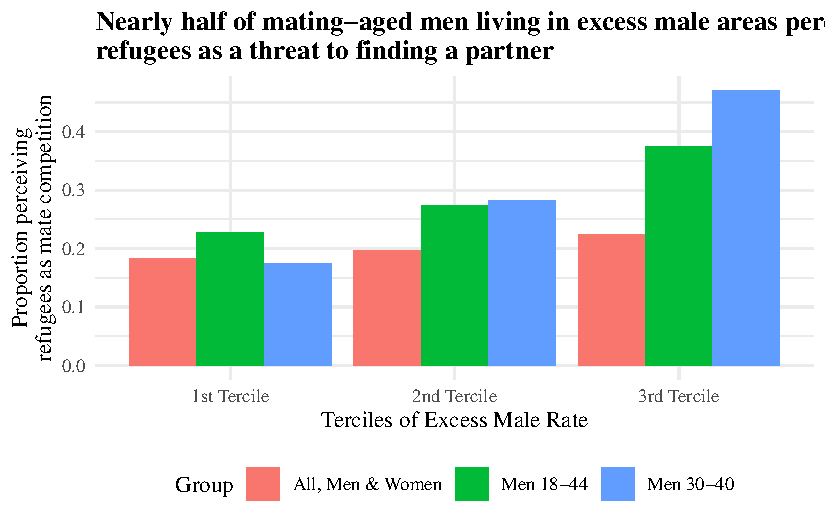
\includegraphics{paper_files/figure-pdf/fig-excess-1.pdf}

}

\caption{\label{fig-excess}look at deez}

\end{figure}

\#\#Figure 2 add prevent bar

\#\#Table 1 have it coded in completely (check marks), better
description of meanings, labels of models (model1, model2,\ldots)

\begin{table}

\caption{\textbf{?(caption)}}\begin{minipage}[t]{\linewidth}

{\centering 

\begin{verbatim}

Call:
lm(formula = only_means ~ mate_compete, data = survey_w4)

Residuals:
    Min      1Q  Median      3Q     Max 
-1.6804 -0.3694 -0.3694  0.6306  2.6306 

Coefficients:
             Estimate Std. Error t value Pr(>|t|)    
(Intercept)   0.93235    0.03302   28.24   <2e-16 ***
mate_compete  0.43702    0.01635   26.73   <2e-16 ***
---
Signif. codes:  0 '***' 0.001 '**' 0.01 '*' 0.05 '.' 0.1 ' ' 1

Residual standard error: 0.7993 on 3017 degrees of freedom
Multiple R-squared:  0.1915,    Adjusted R-squared:  0.1912 
F-statistic: 714.6 on 1 and 3017 DF,  p-value: < 2.2e-16
\end{verbatim}

}

\end{minipage}%
\newline
\begin{minipage}[t]{\linewidth}

{\centering 

\begin{verbatim}

Call:
lm(formula = only_means ~ mate_compete + job_compete + life_satisfaction, 
    data = survey_w4)

Residuals:
    Min      1Q  Median      3Q     Max 
-1.8275 -0.4783 -0.1842  0.3171  2.8452 

Coefficients:
                   Estimate Std. Error t value Pr(>|t|)    
(Intercept)        0.788623   0.057849   13.63   <2e-16 ***
mate_compete       0.263437   0.020261   13.00   <2e-16 ***
job_compete        0.249956   0.018672   13.39   <2e-16 ***
life_satisfaction -0.014725   0.006292   -2.34   0.0193 *  
---
Signif. codes:  0 '***' 0.001 '**' 0.01 '*' 0.05 '.' 0.1 ' ' 1

Residual standard error: 0.7751 on 3015 degrees of freedom
Multiple R-squared:  0.2403,    Adjusted R-squared:  0.2395 
F-statistic: 317.9 on 3 and 3015 DF,  p-value: < 2.2e-16
\end{verbatim}

}

\end{minipage}%
\newline
\begin{minipage}[t]{\linewidth}

{\centering 

\begin{verbatim}

Call:
lm(formula = only_means ~ mate_compete + job_compete + life_satisfaction + 
    factor(age_group) + factor(gender) + factor(state) + factor(citizenship) + 
    factor(marital) + factor(religion) + eduyrs + factor(occupation) + 
    factor(income) + factor(household_size) + factor(self_econ), 
    data = survey_w4)

Residuals:
    Min      1Q  Median      3Q     Max 
-2.2372 -0.4980 -0.1414  0.4129  2.8508 

Coefficients:
                                                                                    Estimate
(Intercept)                                                                        1.5261167
mate_compete                                                                       0.2361496
job_compete                                                                        0.2357615
life_satisfaction                                                                 -0.0136184
factor(age_group)30-39                                                            -0.1323382
factor(age_group)40-49                                                            -0.2088373
factor(age_group)50-59                                                            -0.2875600
factor(age_group)60 and older                                                     -0.3362005
factor(gender)Male                                                                 0.0246837
factor(state)Bayern                                                                0.0096506
factor(state)Berlin                                                                0.0105754
factor(state)Brandenburg                                                          -0.1571611
factor(state)Bremen                                                               -0.1266335
factor(state)Hamburg                                                              -0.0207842
factor(state)Hessen                                                               -0.1207275
factor(state)Mecklenburg-Vorpommern                                               -0.0848947
factor(state)Niedersachsen                                                        -0.0993283
factor(state)Nordrhein-Westfalen                                                  -0.0299069
factor(state)Rheinland-Pfalz                                                      -0.1178332
factor(state)Saarland                                                             -0.0264286
factor(state)Sachsen                                                              -0.0357306
factor(state)Sachsen-Anhalt                                                       -0.0193135
factor(state)Schleswig-Holstein                                                   -0.2401777
factor(state)Th<fc>ringen                                                          0.0089904
factor(citizenship)1                                                              -0.0620992
factor(marital)Married                                                            -0.0265749
factor(marital)Registered partnership                                             -0.0167852
factor(marital)Single, without partner                                            -0.1149664
factor(marital)Widowed                                                             0.0461847
factor(marital)With partner, living together                                      -0.0181225
factor(marital)With partner, not living together                                  -0.0324757
factor(religion)Eastern Orthodox                                                   0.3020609
factor(religion)Eastern religion (Buddhism, Hinduism, Sikhism, Shinto, Tao, etc.)  0.0243803
factor(religion)Jewish                                                             0.1096931
factor(religion)Muslim                                                            -0.0308881
factor(religion)No answer                                                          0.1542223
factor(religion)No, I don't feel close to any religion                             0.0269523
factor(religion)Other Christian                                                    0.0150578
factor(religion)Other non-Christian religion                                       0.4173617
factor(religion)Other Protestant                                                   0.8091199
factor(religion)Protestant                                                        -0.0370041
factor(religion)Protestant Free Church                                             0.0044979
factor(religion)Roman Catholic                                                     0.0235846
eduyrs                                                                            -0.0179429
factor(occupation)Employee in high position                                        0.0544849
factor(occupation)Employee in low / medium position                                0.1073163
factor(occupation)Homemaker                                                        0.0008558
factor(occupation)In schooling / vocational training, student                     -0.0681479
factor(occupation)Other                                                            0.2277531
factor(occupation)Parental leave                                                   0.1948682
factor(occupation)Permanently sick or disabled                                    -0.1565026
factor(occupation)Retired                                                          0.1064025
factor(occupation)Self-employed / freelancer                                       0.1179710
factor(occupation)Senior civil servant                                             0.0181488
factor(occupation)Senior civil servant <96> highest level                         -0.0074663
factor(occupation)Skilled worker                                                   0.2035033
factor(occupation)Unemployed / seeking work                                        0.0096189
factor(occupation)Unskilled worker                                                 0.1808693
factor(income)1,500 to below 2,000 <80>                                            0.0682629
factor(income)2,000 to below 2,500 <80>                                            0.0642248
factor(income)2,500 to below 3,000 <80>                                           -0.0198122
factor(income)3,000 to below 3,500 <80>                                            0.0982123
factor(income)3,500 to below 4,000 <80>                                            0.1578954
factor(income)4,000 to below 4,500 <80>                                            0.0093018
factor(income)4,500 to below 5,000 <80>                                            0.1768821
factor(income)5,000 or more <80>                                                   0.1339431
factor(income)500 to below 1,000 <80>                                             -0.0417322
factor(income)below 500 <80>                                                      -0.0677320
factor(income)No answer                                                           -0.0352015
factor(household_size)2                                                            0.0361567
factor(household_size)3                                                            0.0404118
factor(household_size)4                                                            0.0289028
factor(household_size)5                                                            0.0161021
factor(household_size)6                                                            0.3162084
factor(household_size)7                                                            0.0387091
factor(household_size)8                                                            0.7653693
factor(household_size)12                                                          -0.0288555
factor(self_econ)1                                                                 0.0023263
factor(self_econ)10 ( TOP )                                                        0.3701857
factor(self_econ)2                                                                -0.0247663
factor(self_econ)3                                                                -0.1996112
factor(self_econ)4                                                                -0.1477246
factor(self_econ)5                                                                -0.2255729
factor(self_econ)6                                                                -0.2788824
factor(self_econ)7                                                                -0.3420289
factor(self_econ)8                                                                -0.2083474
factor(self_econ)9                                                                -0.1723641
                                                                                  Std. Error
(Intercept)                                                                        0.2554044
mate_compete                                                                       0.0205981
job_compete                                                                        0.0189414
life_satisfaction                                                                  0.0069537
factor(age_group)30-39                                                             0.0524772
factor(age_group)40-49                                                             0.0525367
factor(age_group)50-59                                                             0.0535204
factor(age_group)60 and older                                                      0.0678073
factor(gender)Male                                                                 0.0299341
factor(state)Bayern                                                                0.0531435
factor(state)Berlin                                                                0.0775641
factor(state)Brandenburg                                                           0.0895704
factor(state)Bremen                                                                0.1530629
factor(state)Hamburg                                                               0.1015866
factor(state)Hessen                                                                0.0647348
factor(state)Mecklenburg-Vorpommern                                                0.1034759
factor(state)Niedersachsen                                                         0.0606795
factor(state)Nordrhein-Westfalen                                                   0.0500592
factor(state)Rheinland-Pfalz                                                       0.0749877
factor(state)Saarland                                                              0.1293265
factor(state)Sachsen                                                               0.0734480
factor(state)Sachsen-Anhalt                                                        0.0926676
factor(state)Schleswig-Holstein                                                    0.0862204
factor(state)Th<fc>ringen                                                          0.0957350
factor(citizenship)1                                                               0.1063941
factor(marital)Married                                                             0.0655813
factor(marital)Registered partnership                                              0.1932772
factor(marital)Single, without partner                                             0.0616006
factor(marital)Widowed                                                             0.0960245
factor(marital)With partner, living together                                       0.0721296
factor(marital)With partner, not living together                                   0.0734540
factor(religion)Eastern Orthodox                                                   0.1944027
factor(religion)Eastern religion (Buddhism, Hinduism, Sikhism, Shinto, Tao, etc.)  0.1321096
factor(religion)Jewish                                                             0.3502700
factor(religion)Muslim                                                             0.1751062
factor(religion)No answer                                                          0.1236346
factor(religion)No, I don't feel close to any religion                             0.0610867
factor(religion)Other Christian                                                    0.1708280
factor(religion)Other non-Christian religion                                       0.2389481
factor(religion)Other Protestant                                                   0.3894084
factor(religion)Protestant                                                         0.0638178
factor(religion)Protestant Free Church                                             0.1147698
factor(religion)Roman Catholic                                                     0.0655525
eduyrs                                                                             0.0041846
factor(occupation)Employee in high position                                        0.1186516
factor(occupation)Employee in low / medium position                                0.1143253
factor(occupation)Homemaker                                                        0.1306711
factor(occupation)In schooling / vocational training, student                      0.1272969
factor(occupation)Other                                                            0.1938874
factor(occupation)Parental leave                                                   0.1822145
factor(occupation)Permanently sick or disabled                                     0.1568823
factor(occupation)Retired                                                          0.1212555
factor(occupation)Self-employed / freelancer                                       0.1251424
factor(occupation)Senior civil servant                                             0.1712732
factor(occupation)Senior civil servant <96> highest level                          0.1513589
factor(occupation)Skilled worker                                                   0.1224862
factor(occupation)Unemployed / seeking work                                        0.1399229
factor(occupation)Unskilled worker                                                 0.1283195
factor(income)1,500 to below 2,000 <80>                                            0.0578960
factor(income)2,000 to below 2,500 <80>                                            0.0603012
factor(income)2,500 to below 3,000 <80>                                            0.0631011
factor(income)3,000 to below 3,500 <80>                                            0.0692386
factor(income)3,500 to below 4,000 <80>                                            0.0735177
factor(income)4,000 to below 4,500 <80>                                            0.0843321
factor(income)4,500 to below 5,000 <80>                                            0.0933501
factor(income)5,000 or more <80>                                                   0.0868492
factor(income)500 to below 1,000 <80>                                              0.0672287
factor(income)below 500 <80>                                                       0.1010999
factor(income)No answer                                                            0.0649465
factor(household_size)2                                                            0.0511259
factor(household_size)3                                                            0.0574134
factor(household_size)4                                                            0.0647219
factor(household_size)5                                                            0.1045545
factor(household_size)6                                                            0.1793375
factor(household_size)7                                                            0.3181027
factor(household_size)8                                                            0.3876451
factor(household_size)12                                                           0.7760703
factor(self_econ)1                                                                 0.2077039
factor(self_econ)10 ( TOP )                                                        0.2423474
factor(self_econ)2                                                                 0.1727396
factor(self_econ)3                                                                 0.1618266
factor(self_econ)4                                                                 0.1624732
factor(self_econ)5                                                                 0.1601877
factor(self_econ)6                                                                 0.1616313
factor(self_econ)7                                                                 0.1630053
factor(self_econ)8                                                                 0.1681510
factor(self_econ)9                                                                 0.2019690
                                                                                  t value
(Intercept)                                                                         5.975
mate_compete                                                                       11.465
job_compete                                                                        12.447
life_satisfaction                                                                  -1.958
factor(age_group)30-39                                                             -2.522
factor(age_group)40-49                                                             -3.975
factor(age_group)50-59                                                             -5.373
factor(age_group)60 and older                                                      -4.958
factor(gender)Male                                                                  0.825
factor(state)Bayern                                                                 0.182
factor(state)Berlin                                                                 0.136
factor(state)Brandenburg                                                           -1.755
factor(state)Bremen                                                                -0.827
factor(state)Hamburg                                                               -0.205
factor(state)Hessen                                                                -1.865
factor(state)Mecklenburg-Vorpommern                                                -0.820
factor(state)Niedersachsen                                                         -1.637
factor(state)Nordrhein-Westfalen                                                   -0.597
factor(state)Rheinland-Pfalz                                                       -1.571
factor(state)Saarland                                                              -0.204
factor(state)Sachsen                                                               -0.486
factor(state)Sachsen-Anhalt                                                        -0.208
factor(state)Schleswig-Holstein                                                    -2.786
factor(state)Th<fc>ringen                                                           0.094
factor(citizenship)1                                                               -0.584
factor(marital)Married                                                             -0.405
factor(marital)Registered partnership                                              -0.087
factor(marital)Single, without partner                                             -1.866
factor(marital)Widowed                                                              0.481
factor(marital)With partner, living together                                       -0.251
factor(marital)With partner, not living together                                   -0.442
factor(religion)Eastern Orthodox                                                    1.554
factor(religion)Eastern religion (Buddhism, Hinduism, Sikhism, Shinto, Tao, etc.)   0.185
factor(religion)Jewish                                                              0.313
factor(religion)Muslim                                                             -0.176
factor(religion)No answer                                                           1.247
factor(religion)No, I don't feel close to any religion                              0.441
factor(religion)Other Christian                                                     0.088
factor(religion)Other non-Christian religion                                        1.747
factor(religion)Other Protestant                                                    2.078
factor(religion)Protestant                                                         -0.580
factor(religion)Protestant Free Church                                              0.039
factor(religion)Roman Catholic                                                      0.360
eduyrs                                                                             -4.288
factor(occupation)Employee in high position                                         0.459
factor(occupation)Employee in low / medium position                                 0.939
factor(occupation)Homemaker                                                         0.007
factor(occupation)In schooling / vocational training, student                      -0.535
factor(occupation)Other                                                             1.175
factor(occupation)Parental leave                                                    1.069
factor(occupation)Permanently sick or disabled                                     -0.998
factor(occupation)Retired                                                           0.878
factor(occupation)Self-employed / freelancer                                        0.943
factor(occupation)Senior civil servant                                              0.106
factor(occupation)Senior civil servant <96> highest level                          -0.049
factor(occupation)Skilled worker                                                    1.661
factor(occupation)Unemployed / seeking work                                         0.069
factor(occupation)Unskilled worker                                                  1.410
factor(income)1,500 to below 2,000 <80>                                             1.179
factor(income)2,000 to below 2,500 <80>                                             1.065
factor(income)2,500 to below 3,000 <80>                                            -0.314
factor(income)3,000 to below 3,500 <80>                                             1.418
factor(income)3,500 to below 4,000 <80>                                             2.148
factor(income)4,000 to below 4,500 <80>                                             0.110
factor(income)4,500 to below 5,000 <80>                                             1.895
factor(income)5,000 or more <80>                                                    1.542
factor(income)500 to below 1,000 <80>                                              -0.621
factor(income)below 500 <80>                                                       -0.670
factor(income)No answer                                                            -0.542
factor(household_size)2                                                             0.707
factor(household_size)3                                                             0.704
factor(household_size)4                                                             0.447
factor(household_size)5                                                             0.154
factor(household_size)6                                                             1.763
factor(household_size)7                                                             0.122
factor(household_size)8                                                             1.974
factor(household_size)12                                                           -0.037
factor(self_econ)1                                                                  0.011
factor(self_econ)10 ( TOP )                                                         1.528
factor(self_econ)2                                                                 -0.143
factor(self_econ)3                                                                 -1.233
factor(self_econ)4                                                                 -0.909
factor(self_econ)5                                                                 -1.408
factor(self_econ)6                                                                 -1.725
factor(self_econ)7                                                                 -2.098
factor(self_econ)8                                                                 -1.239
factor(self_econ)9                                                                 -0.853
                                                                                  Pr(>|t|)
(Intercept)                                                                       2.57e-09
mate_compete                                                                       < 2e-16
job_compete                                                                        < 2e-16
life_satisfaction                                                                  0.05028
factor(age_group)30-39                                                             0.01173
factor(age_group)40-49                                                            7.21e-05
factor(age_group)50-59                                                            8.36e-08
factor(age_group)60 and older                                                     7.52e-07
factor(gender)Male                                                                 0.40966
factor(state)Bayern                                                                0.85591
factor(state)Berlin                                                                0.89156
factor(state)Brandenburg                                                           0.07943
factor(state)Bremen                                                                0.40812
factor(state)Hamburg                                                               0.83790
factor(state)Hessen                                                                0.06229
factor(state)Mecklenburg-Vorpommern                                                0.41204
factor(state)Niedersachsen                                                         0.10175
factor(state)Nordrhein-Westfalen                                                   0.55027
factor(state)Rheinland-Pfalz                                                       0.11621
factor(state)Saarland                                                              0.83809
factor(state)Sachsen                                                               0.62667
factor(state)Sachsen-Anhalt                                                        0.83492
factor(state)Schleswig-Holstein                                                    0.00538
factor(state)Th<fc>ringen                                                          0.92519
factor(citizenship)1                                                               0.55949
factor(marital)Married                                                             0.68534
factor(marital)Registered partnership                                              0.93080
factor(marital)Single, without partner                                             0.06210
factor(marital)Widowed                                                             0.63058
factor(marital)With partner, living together                                       0.80164
factor(marital)With partner, not living together                                   0.65843
factor(religion)Eastern Orthodox                                                   0.12034
factor(religion)Eastern religion (Buddhism, Hinduism, Sikhism, Shinto, Tao, etc.)  0.85360
factor(religion)Jewish                                                             0.75418
factor(religion)Muslim                                                             0.85999
factor(religion)No answer                                                          0.21235
factor(religion)No, I don't feel close to any religion                             0.65909
factor(religion)Other Christian                                                    0.92977
factor(religion)Other non-Christian religion                                       0.08080
factor(religion)Other Protestant                                                   0.03781
factor(religion)Protestant                                                         0.56207
factor(religion)Protestant Free Church                                             0.96874
factor(religion)Roman Catholic                                                     0.71904
eduyrs                                                                            1.86e-05
factor(occupation)Employee in high position                                        0.64612
factor(occupation)Employee in low / medium position                                0.34797
factor(occupation)Homemaker                                                        0.99477
factor(occupation)In schooling / vocational training, student                      0.59245
factor(occupation)Other                                                            0.24022
factor(occupation)Parental leave                                                   0.28496
factor(occupation)Permanently sick or disabled                                     0.31857
factor(occupation)Retired                                                          0.38028
factor(occupation)Self-employed / freelancer                                       0.34592
factor(occupation)Senior civil servant                                             0.91562
factor(occupation)Senior civil servant <96> highest level                          0.96066
factor(occupation)Skilled worker                                                   0.09673
factor(occupation)Unemployed / seeking work                                        0.94520
factor(occupation)Unskilled worker                                                 0.15879
factor(income)1,500 to below 2,000 <80>                                            0.23847
factor(income)2,000 to below 2,500 <80>                                            0.28693
factor(income)2,500 to below 3,000 <80>                                            0.75356
factor(income)3,000 to below 3,500 <80>                                            0.15616
factor(income)3,500 to below 4,000 <80>                                            0.03182
factor(income)4,000 to below 4,500 <80>                                            0.91218
factor(income)4,500 to below 5,000 <80>                                            0.05821
factor(income)5,000 or more <80>                                                   0.12312
factor(income)500 to below 1,000 <80>                                              0.53481
factor(income)below 500 <80>                                                       0.50294
factor(income)No answer                                                            0.58785
factor(household_size)2                                                            0.47949
factor(household_size)3                                                            0.48157
factor(household_size)4                                                            0.65522
factor(household_size)5                                                            0.87761
factor(household_size)6                                                            0.07797
factor(household_size)7                                                            0.90315
factor(household_size)8                                                            0.04843
factor(household_size)12                                                           0.97034
factor(self_econ)1                                                                 0.99106
factor(self_econ)10 ( TOP )                                                        0.12674
factor(self_econ)2                                                                 0.88601
factor(self_econ)3                                                                 0.21749
factor(self_econ)4                                                                 0.36331
factor(self_econ)5                                                                 0.15918
factor(self_econ)6                                                                 0.08456
factor(self_econ)7                                                                 0.03597
factor(self_econ)8                                                                 0.21543
factor(self_econ)9                                                                 0.39350
                                                                                     
(Intercept)                                                                       ***
mate_compete                                                                      ***
job_compete                                                                       ***
life_satisfaction                                                                 .  
factor(age_group)30-39                                                            *  
factor(age_group)40-49                                                            ***
factor(age_group)50-59                                                            ***
factor(age_group)60 and older                                                     ***
factor(gender)Male                                                                   
factor(state)Bayern                                                                  
factor(state)Berlin                                                                  
factor(state)Brandenburg                                                          .  
factor(state)Bremen                                                                  
factor(state)Hamburg                                                                 
factor(state)Hessen                                                               .  
factor(state)Mecklenburg-Vorpommern                                                  
factor(state)Niedersachsen                                                           
factor(state)Nordrhein-Westfalen                                                     
factor(state)Rheinland-Pfalz                                                         
factor(state)Saarland                                                                
factor(state)Sachsen                                                                 
factor(state)Sachsen-Anhalt                                                          
factor(state)Schleswig-Holstein                                                   ** 
factor(state)Th<fc>ringen                                                            
factor(citizenship)1                                                                 
factor(marital)Married                                                               
factor(marital)Registered partnership                                                
factor(marital)Single, without partner                                            .  
factor(marital)Widowed                                                               
factor(marital)With partner, living together                                         
factor(marital)With partner, not living together                                     
factor(religion)Eastern Orthodox                                                     
factor(religion)Eastern religion (Buddhism, Hinduism, Sikhism, Shinto, Tao, etc.)    
factor(religion)Jewish                                                               
factor(religion)Muslim                                                               
factor(religion)No answer                                                            
factor(religion)No, I don't feel close to any religion                               
factor(religion)Other Christian                                                      
factor(religion)Other non-Christian religion                                      .  
factor(religion)Other Protestant                                                  *  
factor(religion)Protestant                                                           
factor(religion)Protestant Free Church                                               
factor(religion)Roman Catholic                                                       
eduyrs                                                                            ***
factor(occupation)Employee in high position                                          
factor(occupation)Employee in low / medium position                                  
factor(occupation)Homemaker                                                          
factor(occupation)In schooling / vocational training, student                        
factor(occupation)Other                                                              
factor(occupation)Parental leave                                                     
factor(occupation)Permanently sick or disabled                                       
factor(occupation)Retired                                                            
factor(occupation)Self-employed / freelancer                                         
factor(occupation)Senior civil servant                                               
factor(occupation)Senior civil servant <96> highest level                            
factor(occupation)Skilled worker                                                  .  
factor(occupation)Unemployed / seeking work                                          
factor(occupation)Unskilled worker                                                   
factor(income)1,500 to below 2,000 <80>                                              
factor(income)2,000 to below 2,500 <80>                                              
factor(income)2,500 to below 3,000 <80>                                              
factor(income)3,000 to below 3,500 <80>                                              
factor(income)3,500 to below 4,000 <80>                                           *  
factor(income)4,000 to below 4,500 <80>                                              
factor(income)4,500 to below 5,000 <80>                                           .  
factor(income)5,000 or more <80>                                                     
factor(income)500 to below 1,000 <80>                                                
factor(income)below 500 <80>                                                         
factor(income)No answer                                                              
factor(household_size)2                                                              
factor(household_size)3                                                              
factor(household_size)4                                                              
factor(household_size)5                                                              
factor(household_size)6                                                           .  
factor(household_size)7                                                              
factor(household_size)8                                                           *  
factor(household_size)12                                                             
factor(self_econ)1                                                                   
factor(self_econ)10 ( TOP )                                                          
factor(self_econ)2                                                                   
factor(self_econ)3                                                                   
factor(self_econ)4                                                                   
factor(self_econ)5                                                                   
factor(self_econ)6                                                                .  
factor(self_econ)7                                                                *  
factor(self_econ)8                                                                   
factor(self_econ)9                                                                   
---
Signif. codes:  0 '***' 0.001 '**' 0.01 '*' 0.05 '.' 0.1 ' ' 1

Residual standard error: 0.7602 on 2921 degrees of freedom
  (11 observations deleted due to missingness)
Multiple R-squared:  0.2883,    Adjusted R-squared:  0.2673 
F-statistic: 13.76 on 86 and 2921 DF,  p-value: < 2.2e-16
\end{verbatim}

}

\end{minipage}%
\newline
\begin{minipage}[t]{\linewidth}

{\centering 

\begin{verbatim}

Call:
lm(formula = only_means ~ mate_compete + job_compete + life_satisfaction + 
    factor(age_group) + factor(gender) + factor(state) + factor(citizenship) + 
    factor(marital) + factor(religion) + eduyrs + factor(occupation) + 
    factor(income) + factor(household_size) + factor(self_econ) + 
    factor(ref_integrating) + factor(ref_citizenship) + factor(ref_reduce) + 
    factor(ref_moredone) + factor(ref_cultgiveup) + factor(ref_economy) + 
    factor(ref_crime) + factor(ref_terror), data = survey_w4)

Residuals:
     Min       1Q   Median       3Q      Max 
-2.33950 -0.43723 -0.07933  0.40274  2.57815 

Coefficients:
                                                                                    Estimate
(Intercept)                                                                        1.4151661
mate_compete                                                                       0.2064398
job_compete                                                                        0.0772492
life_satisfaction                                                                 -0.0034333
factor(age_group)30-39                                                            -0.1800382
factor(age_group)40-49                                                            -0.2771281
factor(age_group)50-59                                                            -0.3621001
factor(age_group)60 and older                                                     -0.3427140
factor(gender)Male                                                                 0.0528358
factor(state)Bayern                                                               -0.0168110
factor(state)Berlin                                                               -0.0022712
factor(state)Brandenburg                                                          -0.1023227
factor(state)Bremen                                                               -0.1252298
factor(state)Hamburg                                                              -0.0139759
factor(state)Hessen                                                               -0.0930806
factor(state)Mecklenburg-Vorpommern                                               -0.1007781
factor(state)Niedersachsen                                                        -0.1052118
factor(state)Nordrhein-Westfalen                                                  -0.0277382
factor(state)Rheinland-Pfalz                                                      -0.1137440
factor(state)Saarland                                                              0.0226726
factor(state)Sachsen                                                              -0.0812750
factor(state)Sachsen-Anhalt                                                       -0.0811416
factor(state)Schleswig-Holstein                                                   -0.1692556
factor(state)Th<fc>ringen                                                         -0.0075831
factor(citizenship)1                                                              -0.0830612
factor(marital)Married                                                            -0.0450582
factor(marital)Registered partnership                                              0.0407631
factor(marital)Single, without partner                                            -0.0937777
factor(marital)Widowed                                                             0.0618683
factor(marital)With partner, living together                                      -0.0367860
factor(marital)With partner, not living together                                  -0.0614547
factor(religion)Eastern Orthodox                                                   0.1563838
factor(religion)Eastern religion (Buddhism, Hinduism, Sikhism, Shinto, Tao, etc.) -0.0058884
factor(religion)Jewish                                                            -0.1431401
factor(religion)Muslim                                                             0.0484324
factor(religion)No answer                                                          0.2155422
factor(religion)No, I don't feel close to any religion                            -0.0101958
factor(religion)Other Christian                                                    0.0304070
factor(religion)Other non-Christian religion                                       0.4656876
factor(religion)Other Protestant                                                   0.9184341
factor(religion)Protestant                                                        -0.0497784
factor(religion)Protestant Free Church                                            -0.0341501
factor(religion)Roman Catholic                                                    -0.0402042
eduyrs                                                                            -0.0139435
factor(occupation)Employee in high position                                        0.0944912
factor(occupation)Employee in low / medium position                                0.1620263
factor(occupation)Homemaker                                                        0.1060568
factor(occupation)In schooling / vocational training, student                     -0.0135564
factor(occupation)Other                                                            0.1527236
factor(occupation)Parental leave                                                   0.2429040
factor(occupation)Permanently sick or disabled                                    -0.0429614
factor(occupation)Retired                                                          0.1553143
factor(occupation)Self-employed / freelancer                                       0.1383632
factor(occupation)Senior civil servant                                             0.1145521
factor(occupation)Senior civil servant <96> highest level                          0.0044789
factor(occupation)Skilled worker                                                   0.2440006
factor(occupation)Unemployed / seeking work                                        0.0721338
factor(occupation)Unskilled worker                                                 0.1953681
factor(income)1,500 to below 2,000 <80>                                            0.0574870
factor(income)2,000 to below 2,500 <80>                                            0.0441103
factor(income)2,500 to below 3,000 <80>                                           -0.0107667
factor(income)3,000 to below 3,500 <80>                                            0.0816849
factor(income)3,500 to below 4,000 <80>                                            0.1419630
factor(income)4,000 to below 4,500 <80>                                           -0.0317864
factor(income)4,500 to below 5,000 <80>                                            0.1067784
factor(income)5,000 or more <80>                                                   0.0635994
factor(income)500 to below 1,000 <80>                                              0.0054025
factor(income)below 500 <80>                                                      -0.0713828
factor(income)No answer                                                           -0.0215701
factor(household_size)2                                                            0.0390020
factor(household_size)3                                                            0.0374263
factor(household_size)4                                                            0.0128680
factor(household_size)5                                                            0.0255404
factor(household_size)6                                                            0.3629212
factor(household_size)7                                                            0.0311236
factor(household_size)8                                                            0.9534169
factor(household_size)12                                                           0.0946449
factor(self_econ)1                                                                 0.0450179
factor(self_econ)10 ( TOP )                                                        0.3410303
factor(self_econ)2                                                                -0.0716097
factor(self_econ)3                                                                -0.1619218
factor(self_econ)4                                                                -0.0943809
factor(self_econ)5                                                                -0.1249692
factor(self_econ)6                                                                -0.1740985
factor(self_econ)7                                                                -0.2076582
factor(self_econ)8                                                                -0.1147817
factor(self_econ)9                                                                -0.0026089
factor(ref_integrating)2                                                          -0.0584895
factor(ref_integrating)3                                                          -0.0920896
factor(ref_integrating)4                                                           0.0787311
factor(ref_citizenship)2                                                           0.0020023
factor(ref_citizenship)3                                                           0.0893018
factor(ref_citizenship)4                                                           0.1625644
factor(ref_reduce)2                                                               -0.0253236
factor(ref_reduce)3                                                                0.0161913
factor(ref_reduce)4                                                                0.0354256
factor(ref_moredone)2                                                              0.0930468
factor(ref_moredone)3                                                              0.1946747
factor(ref_moredone)4                                                              0.3050254
factor(ref_cultgiveup)2                                                           -0.0124946
factor(ref_cultgiveup)3                                                            0.0145151
factor(ref_cultgiveup)4                                                            0.1506527
factor(ref_economy)2                                                               0.0237472
factor(ref_economy)3                                                              -0.0004069
factor(ref_economy)4                                                               0.1656986
factor(ref_crime)2                                                                 0.0183417
factor(ref_crime)3                                                                 0.0793713
factor(ref_crime)4                                                                 0.2506303
factor(ref_terror)2                                                               -0.0688518
factor(ref_terror)3                                                               -0.0330309
factor(ref_terror)4                                                               -0.0338002
                                                                                  Std. Error
(Intercept)                                                                        0.2515301
mate_compete                                                                       0.0193554
job_compete                                                                        0.0195098
life_satisfaction                                                                  0.0064849
factor(age_group)30-39                                                             0.0488567
factor(age_group)40-49                                                             0.0490349
factor(age_group)50-59                                                             0.0500525
factor(age_group)60 and older                                                      0.0631165
factor(gender)Male                                                                 0.0280562
factor(state)Bayern                                                                0.0493801
factor(state)Berlin                                                                0.0721964
factor(state)Brandenburg                                                           0.0833339
factor(state)Bremen                                                                0.1422711
factor(state)Hamburg                                                               0.0946188
factor(state)Hessen                                                                0.0603533
factor(state)Mecklenburg-Vorpommern                                                0.0961128
factor(state)Niedersachsen                                                         0.0563999
factor(state)Nordrhein-Westfalen                                                   0.0465211
factor(state)Rheinland-Pfalz                                                       0.0699756
factor(state)Saarland                                                              0.1203256
factor(state)Sachsen                                                               0.0683059
factor(state)Sachsen-Anhalt                                                        0.0862159
factor(state)Schleswig-Holstein                                                    0.0806118
factor(state)Th<fc>ringen                                                          0.0888795
factor(citizenship)1                                                               0.0990261
factor(marital)Married                                                             0.0609256
factor(marital)Registered partnership                                              0.1802184
factor(marital)Single, without partner                                             0.0573060
factor(marital)Widowed                                                             0.0892253
factor(marital)With partner, living together                                       0.0670370
factor(marital)With partner, not living together                                   0.0683764
factor(religion)Eastern Orthodox                                                   0.1814436
factor(religion)Eastern religion (Buddhism, Hinduism, Sikhism, Shinto, Tao, etc.)  0.1228679
factor(religion)Jewish                                                             0.3256577
factor(religion)Muslim                                                             0.1629797
factor(religion)No answer                                                          0.1149377
factor(religion)No, I don't feel close to any religion                             0.0567357
factor(religion)Other Christian                                                    0.1589033
factor(religion)Other non-Christian religion                                       0.2226449
factor(religion)Other Protestant                                                   0.3622242
factor(religion)Protestant                                                         0.0593148
factor(religion)Protestant Free Church                                             0.1067801
factor(religion)Roman Catholic                                                     0.0610012
eduyrs                                                                             0.0038952
factor(occupation)Employee in high position                                        0.1103005
factor(occupation)Employee in low / medium position                                0.1062773
factor(occupation)Homemaker                                                        0.1214494
factor(occupation)In schooling / vocational training, student                      0.1185551
factor(occupation)Other                                                            0.1804818
factor(occupation)Parental leave                                                   0.1694996
factor(occupation)Permanently sick or disabled                                     0.1462215
factor(occupation)Retired                                                          0.1127063
factor(occupation)Self-employed / freelancer                                       0.1164301
factor(occupation)Senior civil servant                                             0.1594372
factor(occupation)Senior civil servant <96> highest level                          0.1408207
factor(occupation)Skilled worker                                                   0.1140456
factor(occupation)Unemployed / seeking work                                        0.1301538
factor(occupation)Unskilled worker                                                 0.1194160
factor(income)1,500 to below 2,000 <80>                                            0.0539531
factor(income)2,000 to below 2,500 <80>                                            0.0562309
factor(income)2,500 to below 3,000 <80>                                            0.0587904
factor(income)3,000 to below 3,500 <80>                                            0.0644401
factor(income)3,500 to below 4,000 <80>                                            0.0685428
factor(income)4,000 to below 4,500 <80>                                            0.0784650
factor(income)4,500 to below 5,000 <80>                                            0.0870454
factor(income)5,000 or more <80>                                                   0.0809028
factor(income)500 to below 1,000 <80>                                              0.0625829
factor(income)below 500 <80>                                                       0.0943084
factor(income)No answer                                                            0.0606862
factor(household_size)2                                                            0.0475270
factor(household_size)3                                                            0.0535197
factor(household_size)4                                                            0.0601753
factor(household_size)5                                                            0.0972482
factor(household_size)6                                                            0.1665592
factor(household_size)7                                                            0.2956540
factor(household_size)8                                                            0.3614691
factor(household_size)12                                                           0.7216723
factor(self_econ)1                                                                 0.1932848
factor(self_econ)10 ( TOP )                                                        0.2258863
factor(self_econ)2                                                                 0.1608335
factor(self_econ)3                                                                 0.1506322
factor(self_econ)4                                                                 0.1513630
factor(self_econ)5                                                                 0.1493085
factor(self_econ)6                                                                 0.1505152
factor(self_econ)7                                                                 0.1519824
factor(self_econ)8                                                                 0.1566626
factor(self_econ)9                                                                 0.1882811
factor(ref_integrating)2                                                           0.0913252
factor(ref_integrating)3                                                           0.0934726
factor(ref_integrating)4                                                           0.0997704
factor(ref_citizenship)2                                                           0.0443872
factor(ref_citizenship)3                                                           0.0492866
factor(ref_citizenship)4                                                           0.0570846
factor(ref_reduce)2                                                                0.0595169
factor(ref_reduce)3                                                                0.0635958
factor(ref_reduce)4                                                                0.0744072
factor(ref_moredone)2                                                              0.0481993
factor(ref_moredone)3                                                              0.0527971
factor(ref_moredone)4                                                              0.0617670
factor(ref_cultgiveup)2                                                            0.0586076
factor(ref_cultgiveup)3                                                            0.0582276
factor(ref_cultgiveup)4                                                            0.0652420
factor(ref_economy)2                                                               0.0548970
factor(ref_economy)3                                                               0.0605714
factor(ref_economy)4                                                               0.0702271
factor(ref_crime)2                                                                 0.0605980
factor(ref_crime)3                                                                 0.0660677
factor(ref_crime)4                                                                 0.0773646
factor(ref_terror)2                                                                0.0568459
factor(ref_terror)3                                                                0.0608409
factor(ref_terror)4                                                                0.0706890
                                                                                  t value
(Intercept)                                                                         5.626
mate_compete                                                                       10.666
job_compete                                                                         3.959
life_satisfaction                                                                  -0.529
factor(age_group)30-39                                                             -3.685
factor(age_group)40-49                                                             -5.652
factor(age_group)50-59                                                             -7.234
factor(age_group)60 and older                                                      -5.430
factor(gender)Male                                                                  1.883
factor(state)Bayern                                                                -0.340
factor(state)Berlin                                                                -0.031
factor(state)Brandenburg                                                           -1.228
factor(state)Bremen                                                                -0.880
factor(state)Hamburg                                                               -0.148
factor(state)Hessen                                                                -1.542
factor(state)Mecklenburg-Vorpommern                                                -1.049
factor(state)Niedersachsen                                                         -1.865
factor(state)Nordrhein-Westfalen                                                   -0.596
factor(state)Rheinland-Pfalz                                                       -1.625
factor(state)Saarland                                                               0.188
factor(state)Sachsen                                                               -1.190
factor(state)Sachsen-Anhalt                                                        -0.941
factor(state)Schleswig-Holstein                                                    -2.100
factor(state)Th<fc>ringen                                                          -0.085
factor(citizenship)1                                                               -0.839
factor(marital)Married                                                             -0.740
factor(marital)Registered partnership                                               0.226
factor(marital)Single, without partner                                             -1.636
factor(marital)Widowed                                                              0.693
factor(marital)With partner, living together                                       -0.549
factor(marital)With partner, not living together                                   -0.899
factor(religion)Eastern Orthodox                                                    0.862
factor(religion)Eastern religion (Buddhism, Hinduism, Sikhism, Shinto, Tao, etc.)  -0.048
factor(religion)Jewish                                                             -0.440
factor(religion)Muslim                                                              0.297
factor(religion)No answer                                                           1.875
factor(religion)No, I don't feel close to any religion                             -0.180
factor(religion)Other Christian                                                     0.191
factor(religion)Other non-Christian religion                                        2.092
factor(religion)Other Protestant                                                    2.536
factor(religion)Protestant                                                         -0.839
factor(religion)Protestant Free Church                                             -0.320
factor(religion)Roman Catholic                                                     -0.659
eduyrs                                                                             -3.580
factor(occupation)Employee in high position                                         0.857
factor(occupation)Employee in low / medium position                                 1.525
factor(occupation)Homemaker                                                         0.873
factor(occupation)In schooling / vocational training, student                      -0.114
factor(occupation)Other                                                             0.846
factor(occupation)Parental leave                                                    1.433
factor(occupation)Permanently sick or disabled                                     -0.294
factor(occupation)Retired                                                           1.378
factor(occupation)Self-employed / freelancer                                        1.188
factor(occupation)Senior civil servant                                              0.718
factor(occupation)Senior civil servant <96> highest level                           0.032
factor(occupation)Skilled worker                                                    2.139
factor(occupation)Unemployed / seeking work                                         0.554
factor(occupation)Unskilled worker                                                  1.636
factor(income)1,500 to below 2,000 <80>                                             1.065
factor(income)2,000 to below 2,500 <80>                                             0.784
factor(income)2,500 to below 3,000 <80>                                            -0.183
factor(income)3,000 to below 3,500 <80>                                             1.268
factor(income)3,500 to below 4,000 <80>                                             2.071
factor(income)4,000 to below 4,500 <80>                                            -0.405
factor(income)4,500 to below 5,000 <80>                                             1.227
factor(income)5,000 or more <80>                                                    0.786
factor(income)500 to below 1,000 <80>                                               0.086
factor(income)below 500 <80>                                                       -0.757
factor(income)No answer                                                            -0.355
factor(household_size)2                                                             0.821
factor(household_size)3                                                             0.699
factor(household_size)4                                                             0.214
factor(household_size)5                                                             0.263
factor(household_size)6                                                             2.179
factor(household_size)7                                                             0.105
factor(household_size)8                                                             2.638
factor(household_size)12                                                            0.131
factor(self_econ)1                                                                  0.233
factor(self_econ)10 ( TOP )                                                         1.510
factor(self_econ)2                                                                 -0.445
factor(self_econ)3                                                                 -1.075
factor(self_econ)4                                                                 -0.624
factor(self_econ)5                                                                 -0.837
factor(self_econ)6                                                                 -1.157
factor(self_econ)7                                                                 -1.366
factor(self_econ)8                                                                 -0.733
factor(self_econ)9                                                                 -0.014
factor(ref_integrating)2                                                           -0.640
factor(ref_integrating)3                                                           -0.985
factor(ref_integrating)4                                                            0.789
factor(ref_citizenship)2                                                            0.045
factor(ref_citizenship)3                                                            1.812
factor(ref_citizenship)4                                                            2.848
factor(ref_reduce)2                                                                -0.425
factor(ref_reduce)3                                                                 0.255
factor(ref_reduce)4                                                                 0.476
factor(ref_moredone)2                                                               1.930
factor(ref_moredone)3                                                               3.687
factor(ref_moredone)4                                                               4.938
factor(ref_cultgiveup)2                                                            -0.213
factor(ref_cultgiveup)3                                                             0.249
factor(ref_cultgiveup)4                                                             2.309
factor(ref_economy)2                                                                0.433
factor(ref_economy)3                                                               -0.007
factor(ref_economy)4                                                                2.359
factor(ref_crime)2                                                                  0.303
factor(ref_crime)3                                                                  1.201
factor(ref_crime)4                                                                  3.240
factor(ref_terror)2                                                                -1.211
factor(ref_terror)3                                                                -0.543
factor(ref_terror)4                                                                -0.478
                                                                                  Pr(>|t|)
(Intercept)                                                                       2.02e-08
mate_compete                                                                       < 2e-16
job_compete                                                                       7.69e-05
life_satisfaction                                                                 0.596549
factor(age_group)30-39                                                            0.000233
factor(age_group)40-49                                                            1.74e-08
factor(age_group)50-59                                                            5.96e-13
factor(age_group)60 and older                                                     6.11e-08
factor(gender)Male                                                                0.059771
factor(state)Bayern                                                               0.733549
factor(state)Berlin                                                               0.974906
factor(state)Brandenburg                                                          0.219598
factor(state)Bremen                                                               0.378814
factor(state)Hamburg                                                              0.882584
factor(state)Hessen                                                               0.123119
factor(state)Mecklenburg-Vorpommern                                               0.294477
factor(state)Niedersachsen                                                        0.062218
factor(state)Nordrhein-Westfalen                                                  0.551055
factor(state)Rheinland-Pfalz                                                      0.104169
factor(state)Saarland                                                             0.850555
factor(state)Sachsen                                                              0.234196
factor(state)Sachsen-Anhalt                                                       0.346709
factor(state)Schleswig-Holstein                                                   0.035847
factor(state)Th<fc>ringen                                                         0.932014
factor(citizenship)1                                                              0.401661
factor(marital)Married                                                            0.459627
factor(marital)Registered partnership                                             0.821072
factor(marital)Single, without partner                                            0.101857
factor(marital)Widowed                                                            0.488118
factor(marital)With partner, living together                                      0.583225
factor(marital)With partner, not living together                                  0.368849
factor(religion)Eastern Orthodox                                                  0.388821
factor(religion)Eastern religion (Buddhism, Hinduism, Sikhism, Shinto, Tao, etc.) 0.961780
factor(religion)Jewish                                                            0.660302
factor(religion)Muslim                                                            0.766359
factor(religion)No answer                                                         0.060852
factor(religion)No, I don't feel close to any religion                            0.857395
factor(religion)Other Christian                                                   0.848260
factor(religion)Other non-Christian religion                                      0.036560
factor(religion)Other Protestant                                                  0.011280
factor(religion)Protestant                                                        0.401413
factor(religion)Protestant Free Church                                            0.749130
factor(religion)Roman Catholic                                                    0.509902
eduyrs                                                                            0.000350
factor(occupation)Employee in high position                                       0.391698
factor(occupation)Employee in low / medium position                               0.127478
factor(occupation)Homemaker                                                       0.382594
factor(occupation)In schooling / vocational training, student                     0.908971
factor(occupation)Other                                                           0.397511
factor(occupation)Parental leave                                                  0.151947
factor(occupation)Permanently sick or disabled                                    0.768924
factor(occupation)Retired                                                         0.168296
factor(occupation)Self-employed / freelancer                                      0.234781
factor(occupation)Senior civil servant                                            0.472521
factor(occupation)Senior civil servant <96> highest level                         0.974629
factor(occupation)Skilled worker                                                  0.032479
factor(occupation)Unemployed / seeking work                                       0.579471
factor(occupation)Unskilled worker                                                0.101942
factor(income)1,500 to below 2,000 <80>                                           0.286739
factor(income)2,000 to below 2,500 <80>                                           0.432840
factor(income)2,500 to below 3,000 <80>                                           0.854703
factor(income)3,000 to below 3,500 <80>                                           0.205039
factor(income)3,500 to below 4,000 <80>                                           0.038432
factor(income)4,000 to below 4,500 <80>                                           0.685431
factor(income)4,500 to below 5,000 <80>                                           0.220036
factor(income)5,000 or more <80>                                                  0.431861
factor(income)500 to below 1,000 <80>                                             0.931214
factor(income)below 500 <80>                                                      0.449166
factor(income)No answer                                                           0.722289
factor(household_size)2                                                           0.411925
factor(household_size)3                                                           0.484420
factor(household_size)4                                                           0.830685
factor(household_size)5                                                           0.792854
factor(household_size)6                                                           0.029417
factor(household_size)7                                                           0.916168
factor(household_size)8                                                           0.008394
factor(household_size)12                                                          0.895668
factor(self_econ)1                                                                0.815848
factor(self_econ)10 ( TOP )                                                       0.131218
factor(self_econ)2                                                                0.656179
factor(self_econ)3                                                                0.282488
factor(self_econ)4                                                                0.532979
factor(self_econ)5                                                                0.402669
factor(self_econ)6                                                                0.247497
factor(self_econ)7                                                                0.171941
factor(self_econ)8                                                                0.463820
factor(self_econ)9                                                                0.988945
factor(ref_integrating)2                                                          0.521929
factor(ref_integrating)3                                                          0.324606
factor(ref_integrating)4                                                          0.430105
factor(ref_citizenship)2                                                          0.964022
factor(ref_citizenship)3                                                          0.070107
factor(ref_citizenship)4                                                          0.004434
factor(ref_reduce)2                                                               0.670514
factor(ref_reduce)3                                                               0.799052
factor(ref_reduce)4                                                               0.634036
factor(ref_moredone)2                                                             0.053647
factor(ref_moredone)3                                                             0.000231
factor(ref_moredone)4                                                             8.33e-07
factor(ref_cultgiveup)2                                                           0.831194
factor(ref_cultgiveup)3                                                           0.803160
factor(ref_cultgiveup)4                                                           0.021006
factor(ref_economy)2                                                              0.665354
factor(ref_economy)3                                                              0.994640
factor(ref_economy)4                                                              0.018367
factor(ref_crime)2                                                                0.762157
factor(ref_crime)3                                                                0.229709
factor(ref_crime)4                                                                0.001211
factor(ref_terror)2                                                               0.225917
factor(ref_terror)3                                                               0.587237
factor(ref_terror)4                                                               0.632577
                                                                                     
(Intercept)                                                                       ***
mate_compete                                                                      ***
job_compete                                                                       ***
life_satisfaction                                                                    
factor(age_group)30-39                                                            ***
factor(age_group)40-49                                                            ***
factor(age_group)50-59                                                            ***
factor(age_group)60 and older                                                     ***
factor(gender)Male                                                                .  
factor(state)Bayern                                                                  
factor(state)Berlin                                                                  
factor(state)Brandenburg                                                             
factor(state)Bremen                                                                  
factor(state)Hamburg                                                                 
factor(state)Hessen                                                                  
factor(state)Mecklenburg-Vorpommern                                                  
factor(state)Niedersachsen                                                        .  
factor(state)Nordrhein-Westfalen                                                     
factor(state)Rheinland-Pfalz                                                         
factor(state)Saarland                                                                
factor(state)Sachsen                                                                 
factor(state)Sachsen-Anhalt                                                          
factor(state)Schleswig-Holstein                                                   *  
factor(state)Th<fc>ringen                                                            
factor(citizenship)1                                                                 
factor(marital)Married                                                               
factor(marital)Registered partnership                                                
factor(marital)Single, without partner                                               
factor(marital)Widowed                                                               
factor(marital)With partner, living together                                         
factor(marital)With partner, not living together                                     
factor(religion)Eastern Orthodox                                                     
factor(religion)Eastern religion (Buddhism, Hinduism, Sikhism, Shinto, Tao, etc.)    
factor(religion)Jewish                                                               
factor(religion)Muslim                                                               
factor(religion)No answer                                                         .  
factor(religion)No, I don't feel close to any religion                               
factor(religion)Other Christian                                                      
factor(religion)Other non-Christian religion                                      *  
factor(religion)Other Protestant                                                  *  
factor(religion)Protestant                                                           
factor(religion)Protestant Free Church                                               
factor(religion)Roman Catholic                                                       
eduyrs                                                                            ***
factor(occupation)Employee in high position                                          
factor(occupation)Employee in low / medium position                                  
factor(occupation)Homemaker                                                          
factor(occupation)In schooling / vocational training, student                        
factor(occupation)Other                                                              
factor(occupation)Parental leave                                                     
factor(occupation)Permanently sick or disabled                                       
factor(occupation)Retired                                                            
factor(occupation)Self-employed / freelancer                                         
factor(occupation)Senior civil servant                                               
factor(occupation)Senior civil servant <96> highest level                            
factor(occupation)Skilled worker                                                  *  
factor(occupation)Unemployed / seeking work                                          
factor(occupation)Unskilled worker                                                   
factor(income)1,500 to below 2,000 <80>                                              
factor(income)2,000 to below 2,500 <80>                                              
factor(income)2,500 to below 3,000 <80>                                              
factor(income)3,000 to below 3,500 <80>                                              
factor(income)3,500 to below 4,000 <80>                                           *  
factor(income)4,000 to below 4,500 <80>                                              
factor(income)4,500 to below 5,000 <80>                                              
factor(income)5,000 or more <80>                                                     
factor(income)500 to below 1,000 <80>                                                
factor(income)below 500 <80>                                                         
factor(income)No answer                                                              
factor(household_size)2                                                              
factor(household_size)3                                                              
factor(household_size)4                                                              
factor(household_size)5                                                              
factor(household_size)6                                                           *  
factor(household_size)7                                                              
factor(household_size)8                                                           ** 
factor(household_size)12                                                             
factor(self_econ)1                                                                   
factor(self_econ)10 ( TOP )                                                          
factor(self_econ)2                                                                   
factor(self_econ)3                                                                   
factor(self_econ)4                                                                   
factor(self_econ)5                                                                   
factor(self_econ)6                                                                   
factor(self_econ)7                                                                   
factor(self_econ)8                                                                   
factor(self_econ)9                                                                   
factor(ref_integrating)2                                                             
factor(ref_integrating)3                                                             
factor(ref_integrating)4                                                             
factor(ref_citizenship)2                                                             
factor(ref_citizenship)3                                                          .  
factor(ref_citizenship)4                                                          ** 
factor(ref_reduce)2                                                                  
factor(ref_reduce)3                                                                  
factor(ref_reduce)4                                                                  
factor(ref_moredone)2                                                             .  
factor(ref_moredone)3                                                             ***
factor(ref_moredone)4                                                             ***
factor(ref_cultgiveup)2                                                              
factor(ref_cultgiveup)3                                                              
factor(ref_cultgiveup)4                                                           *  
factor(ref_economy)2                                                                 
factor(ref_economy)3                                                                 
factor(ref_economy)4                                                              *  
factor(ref_crime)2                                                                   
factor(ref_crime)3                                                                   
factor(ref_crime)4                                                                ** 
factor(ref_terror)2                                                                  
factor(ref_terror)3                                                                  
factor(ref_terror)4                                                                  
---
Signif. codes:  0 '***' 0.001 '**' 0.01 '*' 0.05 '.' 0.1 ' ' 1

Residual standard error: 0.7042 on 2897 degrees of freedom
  (11 observations deleted due to missingness)
Multiple R-squared:  0.3942,    Adjusted R-squared:  0.3712 
F-statistic: 17.14 on 110 and 2897 DF,  p-value: < 2.2e-16
\end{verbatim}

}

\end{minipage}%
\newline
\begin{minipage}[t]{\linewidth}

{\centering 

\begin{verbatim}

Call:
lm(formula = only_means ~ mate_compete + job_compete + life_satisfaction + 
    factor(age_group) + factor(gender) + factor(state) + factor(citizenship) + 
    factor(marital) + factor(religion) + eduyrs + factor(occupation) + 
    factor(income) + factor(household_size) + factor(self_econ) + 
    factor(ref_integrating) + factor(ref_citizenship) + factor(ref_reduce) + 
    factor(ref_moredone) + factor(ref_cultgiveup) + factor(ref_economy) + 
    factor(ref_crime) + factor(ref_terror) + factor(ref_loc_services) + 
    factor(ref_loc_economy) + factor(ref_loc_crime) + factor(ref_loc_culture) + 
    factor(ref_loc_islam) + factor(ref_loc_schools) + factor(ref_loc_housing) + 
    factor(ref_loc_wayoflife), data = survey_w4)

Residuals:
     Min       1Q   Median       3Q      Max 
-2.28589 -0.42763 -0.07577  0.37530  2.41299 

Coefficients:
                                                                                   Estimate
(Intercept)                                                                        1.387754
mate_compete                                                                       0.184842
job_compete                                                                        0.065026
life_satisfaction                                                                 -0.001981
factor(age_group)30-39                                                            -0.182069
factor(age_group)40-49                                                            -0.270879
factor(age_group)50-59                                                            -0.348007
factor(age_group)60 and older                                                     -0.319885
factor(gender)Male                                                                 0.045137
factor(state)Bayern                                                               -0.014849
factor(state)Berlin                                                               -0.025880
factor(state)Brandenburg                                                          -0.094851
factor(state)Bremen                                                               -0.174988
factor(state)Hamburg                                                              -0.025450
factor(state)Hessen                                                               -0.076563
factor(state)Mecklenburg-Vorpommern                                               -0.101540
factor(state)Niedersachsen                                                        -0.105534
factor(state)Nordrhein-Westfalen                                                  -0.041363
factor(state)Rheinland-Pfalz                                                      -0.108869
factor(state)Saarland                                                              0.035308
factor(state)Sachsen                                                              -0.111810
factor(state)Sachsen-Anhalt                                                       -0.076544
factor(state)Schleswig-Holstein                                                   -0.172541
factor(state)Th<fc>ringen                                                         -0.008119
factor(citizenship)1                                                              -0.073865
factor(marital)Married                                                            -0.034389
factor(marital)Registered partnership                                              0.074827
factor(marital)Single, without partner                                            -0.085272
factor(marital)Widowed                                                             0.045649
factor(marital)With partner, living together                                      -0.027059
factor(marital)With partner, not living together                                  -0.070799
factor(religion)Eastern Orthodox                                                   0.126686
factor(religion)Eastern religion (Buddhism, Hinduism, Sikhism, Shinto, Tao, etc.)  0.020587
factor(religion)Jewish                                                            -0.093803
factor(religion)Muslim                                                            -0.003636
factor(religion)No answer                                                          0.202299
factor(religion)No, I don't feel close to any religion                            -0.008282
factor(religion)Other Christian                                                    0.056182
factor(religion)Other non-Christian religion                                       0.432889
factor(religion)Other Protestant                                                   0.915127
factor(religion)Protestant                                                        -0.033163
factor(religion)Protestant Free Church                                            -0.025316
factor(religion)Roman Catholic                                                    -0.041564
eduyrs                                                                            -0.012114
factor(occupation)Employee in high position                                        0.117625
factor(occupation)Employee in low / medium position                                0.186577
factor(occupation)Homemaker                                                        0.134166
factor(occupation)In schooling / vocational training, student                      0.006243
factor(occupation)Other                                                            0.157368
factor(occupation)Parental leave                                                   0.266063
factor(occupation)Permanently sick or disabled                                    -0.011630
factor(occupation)Retired                                                          0.181194
factor(occupation)Self-employed / freelancer                                       0.173742
factor(occupation)Senior civil servant                                             0.160352
factor(occupation)Senior civil servant <96> highest level                          0.054833
factor(occupation)Skilled worker                                                   0.273500
factor(occupation)Unemployed / seeking work                                        0.092160
factor(occupation)Unskilled worker                                                 0.198386
factor(income)1,500 to below 2,000 <80>                                            0.067775
factor(income)2,000 to below 2,500 <80>                                            0.050442
factor(income)2,500 to below 3,000 <80>                                           -0.002711
factor(income)3,000 to below 3,500 <80>                                            0.091559
factor(income)3,500 to below 4,000 <80>                                            0.145937
factor(income)4,000 to below 4,500 <80>                                           -0.037090
factor(income)4,500 to below 5,000 <80>                                            0.111305
factor(income)5,000 or more <80>                                                   0.048604
factor(income)500 to below 1,000 <80>                                              0.010841
factor(income)below 500 <80>                                                      -0.064165
factor(income)No answer                                                           -0.014094
factor(household_size)2                                                            0.031601
factor(household_size)3                                                            0.040283
factor(household_size)4                                                            0.011423
factor(household_size)5                                                            0.034738
factor(household_size)6                                                            0.402997
factor(household_size)7                                                            0.049483
factor(household_size)8                                                            0.835222
factor(household_size)12                                                          -0.043483
factor(self_econ)1                                                                 0.027843
factor(self_econ)10 ( TOP )                                                        0.297977
factor(self_econ)2                                                                -0.086263
factor(self_econ)3                                                                -0.177938
factor(self_econ)4                                                                -0.107983
factor(self_econ)5                                                                -0.142663
factor(self_econ)6                                                                -0.190732
factor(self_econ)7                                                                -0.220575
factor(self_econ)8                                                                -0.148608
factor(self_econ)9                                                                -0.040594
factor(ref_integrating)2                                                          -0.038964
factor(ref_integrating)3                                                          -0.069229
factor(ref_integrating)4                                                           0.092784
factor(ref_citizenship)2                                                          -0.020207
factor(ref_citizenship)3                                                           0.072038
factor(ref_citizenship)4                                                           0.142478
factor(ref_reduce)2                                                               -0.010313
factor(ref_reduce)3                                                                0.032647
factor(ref_reduce)4                                                                0.046473
factor(ref_moredone)2                                                              0.080247
factor(ref_moredone)3                                                              0.183432
factor(ref_moredone)4                                                              0.287400
factor(ref_cultgiveup)2                                                           -0.021182
factor(ref_cultgiveup)3                                                           -0.005407
factor(ref_cultgiveup)4                                                            0.128135
factor(ref_economy)2                                                               0.045647
factor(ref_economy)3                                                               0.034347
factor(ref_economy)4                                                               0.237898
factor(ref_crime)2                                                                -0.003322
factor(ref_crime)3                                                                -0.006056
factor(ref_crime)4                                                                 0.134256
factor(ref_terror)2                                                               -0.097474
factor(ref_terror)3                                                               -0.081778
factor(ref_terror)4                                                               -0.086459
factor(ref_loc_services)2                                                          0.085151
factor(ref_loc_services)3                                                          0.076489
factor(ref_loc_services)4                                                          0.057691
factor(ref_loc_economy)2                                                          -0.118562
factor(ref_loc_economy)3                                                          -0.141965
factor(ref_loc_economy)4                                                          -0.289193
factor(ref_loc_crime)2                                                             0.081347
factor(ref_loc_crime)3                                                             0.247361
factor(ref_loc_crime)4                                                             0.311005
factor(ref_loc_culture)2                                                           0.005145
factor(ref_loc_culture)3                                                           0.029727
factor(ref_loc_culture)4                                                           0.123201
factor(ref_loc_islam)2                                                            -0.012791
factor(ref_loc_islam)3                                                            -0.008482
factor(ref_loc_islam)4                                                            -0.028099
factor(ref_loc_schools)2                                                           0.125425
factor(ref_loc_schools)3                                                           0.055239
factor(ref_loc_schools)4                                                          -0.080557
factor(ref_loc_housing)2                                                           0.013393
factor(ref_loc_housing)3                                                           0.006806
factor(ref_loc_housing)4                                                           0.043241
factor(ref_loc_wayoflife)2                                                        -0.058601
factor(ref_loc_wayoflife)3                                                        -0.034112
factor(ref_loc_wayoflife)4                                                         0.069380
                                                                                  Std. Error
(Intercept)                                                                         0.262204
mate_compete                                                                        0.019474
job_compete                                                                         0.019617
life_satisfaction                                                                   0.006459
factor(age_group)30-39                                                              0.048820
factor(age_group)40-49                                                              0.049006
factor(age_group)50-59                                                              0.050173
factor(age_group)60 and older                                                       0.063119
factor(gender)Male                                                                  0.028182
factor(state)Bayern                                                                 0.049130
factor(state)Berlin                                                                 0.072033
factor(state)Brandenburg                                                            0.083365
factor(state)Bremen                                                                 0.141544
factor(state)Hamburg                                                                0.094059
factor(state)Hessen                                                                 0.060069
factor(state)Mecklenburg-Vorpommern                                                 0.095919
factor(state)Niedersachsen                                                          0.056103
factor(state)Nordrhein-Westfalen                                                    0.046472
factor(state)Rheinland-Pfalz                                                        0.069711
factor(state)Saarland                                                               0.119918
factor(state)Sachsen                                                                0.068392
factor(state)Sachsen-Anhalt                                                         0.086301
factor(state)Schleswig-Holstein                                                     0.080204
factor(state)Th<fc>ringen                                                           0.088737
factor(citizenship)1                                                                0.098314
factor(marital)Married                                                              0.060528
factor(marital)Registered partnership                                               0.179296
factor(marital)Single, without partner                                              0.056928
factor(marital)Widowed                                                              0.089044
factor(marital)With partner, living together                                        0.066601
factor(marital)With partner, not living together                                    0.067956
factor(religion)Eastern Orthodox                                                    0.180688
factor(religion)Eastern religion (Buddhism, Hinduism, Sikhism, Shinto, Tao, etc.)   0.122704
factor(religion)Jewish                                                              0.324268
factor(religion)Muslim                                                              0.162434
factor(religion)No answer                                                           0.114753
factor(religion)No, I don't feel close to any religion                              0.056621
factor(religion)Other Christian                                                     0.158439
factor(religion)Other non-Christian religion                                        0.221911
factor(religion)Other Protestant                                                    0.359856
factor(religion)Protestant                                                          0.059138
factor(religion)Protestant Free Church                                              0.106269
factor(religion)Roman Catholic                                                      0.060897
eduyrs                                                                              0.003893
factor(occupation)Employee in high position                                         0.109611
factor(occupation)Employee in low / medium position                                 0.105633
factor(occupation)Homemaker                                                         0.120917
factor(occupation)In schooling / vocational training, student                       0.118020
factor(occupation)Other                                                             0.179672
factor(occupation)Parental leave                                                    0.168609
factor(occupation)Permanently sick or disabled                                      0.145518
factor(occupation)Retired                                                           0.112067
factor(occupation)Self-employed / freelancer                                        0.115842
factor(occupation)Senior civil servant                                              0.158771
factor(occupation)Senior civil servant <96> highest level                           0.140080
factor(occupation)Skilled worker                                                    0.113337
factor(occupation)Unemployed / seeking work                                         0.129438
factor(occupation)Unskilled worker                                                  0.118724
factor(income)1,500 to below 2,000 <80>                                             0.053728
factor(income)2,000 to below 2,500 <80>                                             0.056110
factor(income)2,500 to below 3,000 <80>                                             0.058685
factor(income)3,000 to below 3,500 <80>                                             0.064161
factor(income)3,500 to below 4,000 <80>                                             0.068273
factor(income)4,000 to below 4,500 <80>                                             0.078326
factor(income)4,500 to below 5,000 <80>                                             0.086701
factor(income)5,000 or more <80>                                                    0.080583
factor(income)500 to below 1,000 <80>                                               0.062313
factor(income)below 500 <80>                                                        0.093748
factor(income)No answer                                                             0.060432
factor(household_size)2                                                             0.047274
factor(household_size)3                                                             0.053260
factor(household_size)4                                                             0.059924
factor(household_size)5                                                             0.096828
factor(household_size)6                                                             0.165850
factor(household_size)7                                                             0.293932
factor(household_size)8                                                             0.361493
factor(household_size)12                                                            0.718824
factor(self_econ)1                                                                  0.192518
factor(self_econ)10 ( TOP )                                                         0.224435
factor(self_econ)2                                                                  0.159861
factor(self_econ)3                                                                  0.149755
factor(self_econ)4                                                                  0.150368
factor(self_econ)5                                                                  0.148375
factor(self_econ)6                                                                  0.149518
factor(self_econ)7                                                                  0.151026
factor(self_econ)8                                                                  0.155678
factor(self_econ)9                                                                  0.187679
factor(ref_integrating)2                                                            0.092362
factor(ref_integrating)3                                                            0.095078
factor(ref_integrating)4                                                            0.101488
factor(ref_citizenship)2                                                            0.044651
factor(ref_citizenship)3                                                            0.049693
factor(ref_citizenship)4                                                            0.058112
factor(ref_reduce)2                                                                 0.059891
factor(ref_reduce)3                                                                 0.064394
factor(ref_reduce)4                                                                 0.075355
factor(ref_moredone)2                                                               0.048435
factor(ref_moredone)3                                                               0.053241
factor(ref_moredone)4                                                               0.062325
factor(ref_cultgiveup)2                                                             0.059003
factor(ref_cultgiveup)3                                                             0.058679
factor(ref_cultgiveup)4                                                             0.065555
factor(ref_economy)2                                                                0.058208
factor(ref_economy)3                                                                0.066322
factor(ref_economy)4                                                                0.077785
factor(ref_crime)2                                                                  0.064486
factor(ref_crime)3                                                                  0.071514
factor(ref_crime)4                                                                  0.083538
factor(ref_terror)2                                                                 0.057788
factor(ref_terror)3                                                                 0.061746
factor(ref_terror)4                                                                 0.071483
factor(ref_loc_services)2                                                           0.067990
factor(ref_loc_services)3                                                           0.068148
factor(ref_loc_services)4                                                           0.076091
factor(ref_loc_economy)2                                                            0.071767
factor(ref_loc_economy)3                                                            0.076688
factor(ref_loc_economy)4                                                            0.086423
factor(ref_loc_crime)2                                                              0.058176
factor(ref_loc_crime)3                                                              0.066240
factor(ref_loc_crime)4                                                              0.079966
factor(ref_loc_culture)2                                                            0.052385
factor(ref_loc_culture)3                                                            0.061227
factor(ref_loc_culture)4                                                            0.073701
factor(ref_loc_islam)2                                                              0.053079
factor(ref_loc_islam)3                                                              0.054982
factor(ref_loc_islam)4                                                              0.066027
factor(ref_loc_schools)2                                                            0.088660
factor(ref_loc_schools)3                                                            0.083185
factor(ref_loc_schools)4                                                            0.084465
factor(ref_loc_housing)2                                                            0.058598
factor(ref_loc_housing)3                                                            0.056425
factor(ref_loc_housing)4                                                            0.060829
factor(ref_loc_wayoflife)2                                                          0.062126
factor(ref_loc_wayoflife)3                                                          0.060857
factor(ref_loc_wayoflife)4                                                          0.070696
                                                                                  t value
(Intercept)                                                                         5.293
mate_compete                                                                        9.492
job_compete                                                                         3.315
life_satisfaction                                                                  -0.307
factor(age_group)30-39                                                             -3.729
factor(age_group)40-49                                                             -5.527
factor(age_group)50-59                                                             -6.936
factor(age_group)60 and older                                                      -5.068
factor(gender)Male                                                                  1.602
factor(state)Bayern                                                                -0.302
factor(state)Berlin                                                                -0.359
factor(state)Brandenburg                                                           -1.138
factor(state)Bremen                                                                -1.236
factor(state)Hamburg                                                               -0.271
factor(state)Hessen                                                                -1.275
factor(state)Mecklenburg-Vorpommern                                                -1.059
factor(state)Niedersachsen                                                         -1.881
factor(state)Nordrhein-Westfalen                                                   -0.890
factor(state)Rheinland-Pfalz                                                       -1.562
factor(state)Saarland                                                               0.294
factor(state)Sachsen                                                               -1.635
factor(state)Sachsen-Anhalt                                                        -0.887
factor(state)Schleswig-Holstein                                                    -2.151
factor(state)Th<fc>ringen                                                          -0.092
factor(citizenship)1                                                               -0.751
factor(marital)Married                                                             -0.568
factor(marital)Registered partnership                                               0.417
factor(marital)Single, without partner                                             -1.498
factor(marital)Widowed                                                              0.513
factor(marital)With partner, living together                                       -0.406
factor(marital)With partner, not living together                                   -1.042
factor(religion)Eastern Orthodox                                                    0.701
factor(religion)Eastern religion (Buddhism, Hinduism, Sikhism, Shinto, Tao, etc.)   0.168
factor(religion)Jewish                                                             -0.289
factor(religion)Muslim                                                             -0.022
factor(religion)No answer                                                           1.763
factor(religion)No, I don't feel close to any religion                             -0.146
factor(religion)Other Christian                                                     0.355
factor(religion)Other non-Christian religion                                        1.951
factor(religion)Other Protestant                                                    2.543
factor(religion)Protestant                                                         -0.561
factor(religion)Protestant Free Church                                             -0.238
factor(religion)Roman Catholic                                                     -0.683
eduyrs                                                                             -3.112
factor(occupation)Employee in high position                                         1.073
factor(occupation)Employee in low / medium position                                 1.766
factor(occupation)Homemaker                                                         1.110
factor(occupation)In schooling / vocational training, student                       0.053
factor(occupation)Other                                                             0.876
factor(occupation)Parental leave                                                    1.578
factor(occupation)Permanently sick or disabled                                     -0.080
factor(occupation)Retired                                                           1.617
factor(occupation)Self-employed / freelancer                                        1.500
factor(occupation)Senior civil servant                                              1.010
factor(occupation)Senior civil servant <96> highest level                           0.391
factor(occupation)Skilled worker                                                    2.413
factor(occupation)Unemployed / seeking work                                         0.712
factor(occupation)Unskilled worker                                                  1.671
factor(income)1,500 to below 2,000 <80>                                             1.261
factor(income)2,000 to below 2,500 <80>                                             0.899
factor(income)2,500 to below 3,000 <80>                                            -0.046
factor(income)3,000 to below 3,500 <80>                                             1.427
factor(income)3,500 to below 4,000 <80>                                             2.138
factor(income)4,000 to below 4,500 <80>                                            -0.474
factor(income)4,500 to below 5,000 <80>                                             1.284
factor(income)5,000 or more <80>                                                    0.603
factor(income)500 to below 1,000 <80>                                               0.174
factor(income)below 500 <80>                                                       -0.684
factor(income)No answer                                                            -0.233
factor(household_size)2                                                             0.668
factor(household_size)3                                                             0.756
factor(household_size)4                                                             0.191
factor(household_size)5                                                             0.359
factor(household_size)6                                                             2.430
factor(household_size)7                                                             0.168
factor(household_size)8                                                             2.310
factor(household_size)12                                                           -0.060
factor(self_econ)1                                                                  0.145
factor(self_econ)10 ( TOP )                                                         1.328
factor(self_econ)2                                                                 -0.540
factor(self_econ)3                                                                 -1.188
factor(self_econ)4                                                                 -0.718
factor(self_econ)5                                                                 -0.962
factor(self_econ)6                                                                 -1.276
factor(self_econ)7                                                                 -1.461
factor(self_econ)8                                                                 -0.955
factor(self_econ)9                                                                 -0.216
factor(ref_integrating)2                                                           -0.422
factor(ref_integrating)3                                                           -0.728
factor(ref_integrating)4                                                            0.914
factor(ref_citizenship)2                                                           -0.453
factor(ref_citizenship)3                                                            1.450
factor(ref_citizenship)4                                                            2.452
factor(ref_reduce)2                                                                -0.172
factor(ref_reduce)3                                                                 0.507
factor(ref_reduce)4                                                                 0.617
factor(ref_moredone)2                                                               1.657
factor(ref_moredone)3                                                               3.445
factor(ref_moredone)4                                                               4.611
factor(ref_cultgiveup)2                                                            -0.359
factor(ref_cultgiveup)3                                                            -0.092
factor(ref_cultgiveup)4                                                             1.955
factor(ref_economy)2                                                                0.784
factor(ref_economy)3                                                                0.518
factor(ref_economy)4                                                                3.058
factor(ref_crime)2                                                                 -0.052
factor(ref_crime)3                                                                 -0.085
factor(ref_crime)4                                                                  1.607
factor(ref_terror)2                                                                -1.687
factor(ref_terror)3                                                                -1.324
factor(ref_terror)4                                                                -1.210
factor(ref_loc_services)2                                                           1.252
factor(ref_loc_services)3                                                           1.122
factor(ref_loc_services)4                                                           0.758
factor(ref_loc_economy)2                                                           -1.652
factor(ref_loc_economy)3                                                           -1.851
factor(ref_loc_economy)4                                                           -3.346
factor(ref_loc_crime)2                                                              1.398
factor(ref_loc_crime)3                                                              3.734
factor(ref_loc_crime)4                                                              3.889
factor(ref_loc_culture)2                                                            0.098
factor(ref_loc_culture)3                                                            0.486
factor(ref_loc_culture)4                                                            1.672
factor(ref_loc_islam)2                                                             -0.241
factor(ref_loc_islam)3                                                             -0.154
factor(ref_loc_islam)4                                                             -0.426
factor(ref_loc_schools)2                                                            1.415
factor(ref_loc_schools)3                                                            0.664
factor(ref_loc_schools)4                                                           -0.954
factor(ref_loc_housing)2                                                            0.229
factor(ref_loc_housing)3                                                            0.121
factor(ref_loc_housing)4                                                            0.711
factor(ref_loc_wayoflife)2                                                         -0.943
factor(ref_loc_wayoflife)3                                                         -0.561
factor(ref_loc_wayoflife)4                                                          0.981
                                                                                  Pr(>|t|)
(Intercept)                                                                       1.30e-07
mate_compete                                                                       < 2e-16
job_compete                                                                       0.000929
life_satisfaction                                                                 0.759074
factor(age_group)30-39                                                            0.000196
factor(age_group)40-49                                                            3.54e-08
factor(age_group)50-59                                                            4.96e-12
factor(age_group)60 and older                                                     4.28e-07
factor(gender)Male                                                                0.109348
factor(state)Bayern                                                               0.762491
factor(state)Berlin                                                               0.719408
factor(state)Brandenburg                                                          0.255305
factor(state)Bremen                                                               0.216457
factor(state)Hamburg                                                              0.786736
factor(state)Hessen                                                               0.202560
factor(state)Mecklenburg-Vorpommern                                               0.289870
factor(state)Niedersachsen                                                        0.060061
factor(state)Nordrhein-Westfalen                                                  0.373507
factor(state)Rheinland-Pfalz                                                      0.118461
factor(state)Saarland                                                             0.768445
factor(state)Sachsen                                                              0.102195
factor(state)Sachsen-Anhalt                                                       0.375186
factor(state)Schleswig-Holstein                                                   0.031538
factor(state)Th<fc>ringen                                                         0.927102
factor(citizenship)1                                                              0.452528
factor(marital)Married                                                            0.569980
factor(marital)Registered partnership                                             0.676464
factor(marital)Single, without partner                                            0.134267
factor(marital)Widowed                                                            0.608229
factor(marital)With partner, living together                                      0.684563
factor(marital)With partner, not living together                                  0.297573
factor(religion)Eastern Orthodox                                                  0.483277
factor(religion)Eastern religion (Buddhism, Hinduism, Sikhism, Shinto, Tao, etc.) 0.866771
factor(religion)Jewish                                                            0.772390
factor(religion)Muslim                                                            0.982142
factor(religion)No answer                                                         0.078022
factor(religion)No, I don't feel close to any religion                            0.883725
factor(religion)Other Christian                                                   0.722919
factor(religion)Other non-Christian religion                                      0.051185
factor(religion)Other Protestant                                                  0.011041
factor(religion)Protestant                                                        0.574995
factor(religion)Protestant Free Church                                            0.811726
factor(religion)Roman Catholic                                                    0.494957
eduyrs                                                                            0.001879
factor(occupation)Employee in high position                                       0.283312
factor(occupation)Employee in low / medium position                               0.077456
factor(occupation)Homemaker                                                       0.267277
factor(occupation)In schooling / vocational training, student                     0.957816
factor(occupation)Other                                                           0.381179
factor(occupation)Parental leave                                                  0.114678
factor(occupation)Permanently sick or disabled                                    0.936305
factor(occupation)Retired                                                         0.106022
factor(occupation)Self-employed / freelancer                                      0.133770
factor(occupation)Senior civil servant                                            0.312600
factor(occupation)Senior civil servant <96> highest level                         0.695501
factor(occupation)Skilled worker                                                  0.015877
factor(occupation)Unemployed / seeking work                                       0.476521
factor(occupation)Unskilled worker                                                0.094834
factor(income)1,500 to below 2,000 <80>                                           0.207249
factor(income)2,000 to below 2,500 <80>                                           0.368733
factor(income)2,500 to below 3,000 <80>                                           0.963154
factor(income)3,000 to below 3,500 <80>                                           0.153679
factor(income)3,500 to below 4,000 <80>                                           0.032637
factor(income)4,000 to below 4,500 <80>                                           0.635869
factor(income)4,500 to below 5,000 <80>                                           0.199320
factor(income)5,000 or more <80>                                                  0.546455
factor(income)500 to below 1,000 <80>                                             0.861900
factor(income)below 500 <80>                                                      0.493750
factor(income)No answer                                                           0.815602
factor(household_size)2                                                           0.503886
factor(household_size)3                                                           0.449505
factor(household_size)4                                                           0.848828
factor(household_size)5                                                           0.719802
factor(household_size)6                                                           0.015164
factor(household_size)7                                                           0.866322
factor(household_size)8                                                           0.020932
factor(household_size)12                                                          0.951768
factor(self_econ)1                                                                0.885018
factor(self_econ)10 ( TOP )                                                       0.184389
factor(self_econ)2                                                                0.589506
factor(self_econ)3                                                                0.234856
factor(self_econ)4                                                                0.472739
factor(self_econ)5                                                                0.336379
factor(self_econ)6                                                                0.202185
factor(self_econ)7                                                                0.144258
factor(self_econ)8                                                                0.339869
factor(self_econ)9                                                                0.828773
factor(ref_integrating)2                                                          0.673162
factor(ref_integrating)3                                                          0.466594
factor(ref_integrating)4                                                          0.360672
factor(ref_citizenship)2                                                          0.650907
factor(ref_citizenship)3                                                          0.147259
factor(ref_citizenship)4                                                          0.014275
factor(ref_reduce)2                                                               0.863292
factor(ref_reduce)3                                                               0.612196
factor(ref_reduce)4                                                               0.537469
factor(ref_moredone)2                                                             0.097671
factor(ref_moredone)3                                                             0.000579
factor(ref_moredone)4                                                             4.18e-06
factor(ref_cultgiveup)2                                                           0.719617
factor(ref_cultgiveup)3                                                           0.926588
factor(ref_cultgiveup)4                                                           0.050727
factor(ref_economy)2                                                              0.432980
factor(ref_economy)3                                                              0.604586
factor(ref_economy)4                                                              0.002246
factor(ref_crime)2                                                                0.958914
factor(ref_crime)3                                                                0.932516
factor(ref_crime)4                                                                0.108136
factor(ref_terror)2                                                               0.091758
factor(ref_terror)3                                                               0.185472
factor(ref_terror)4                                                               0.226568
factor(ref_loc_services)2                                                         0.210527
factor(ref_loc_services)3                                                         0.261790
factor(ref_loc_services)4                                                         0.448404
factor(ref_loc_economy)2                                                          0.098635
factor(ref_loc_economy)3                                                          0.064243
factor(ref_loc_economy)4                                                          0.000830
factor(ref_loc_crime)2                                                            0.162130
factor(ref_loc_crime)3                                                            0.000192
factor(ref_loc_crime)4                                                            0.000103
factor(ref_loc_culture)2                                                          0.921775
factor(ref_loc_culture)3                                                          0.627345
factor(ref_loc_culture)4                                                          0.094706
factor(ref_loc_islam)2                                                            0.809582
factor(ref_loc_islam)3                                                            0.877408
factor(ref_loc_islam)4                                                            0.670451
factor(ref_loc_schools)2                                                          0.157272
factor(ref_loc_schools)3                                                          0.506711
factor(ref_loc_schools)4                                                          0.340300
factor(ref_loc_housing)2                                                          0.819225
factor(ref_loc_housing)3                                                          0.904004
factor(ref_loc_housing)4                                                          0.477235
factor(ref_loc_wayoflife)2                                                        0.345630
factor(ref_loc_wayoflife)3                                                        0.575160
factor(ref_loc_wayoflife)4                                                        0.326484
                                                                                     
(Intercept)                                                                       ***
mate_compete                                                                      ***
job_compete                                                                       ***
life_satisfaction                                                                    
factor(age_group)30-39                                                            ***
factor(age_group)40-49                                                            ***
factor(age_group)50-59                                                            ***
factor(age_group)60 and older                                                     ***
factor(gender)Male                                                                   
factor(state)Bayern                                                                  
factor(state)Berlin                                                                  
factor(state)Brandenburg                                                             
factor(state)Bremen                                                                  
factor(state)Hamburg                                                                 
factor(state)Hessen                                                                  
factor(state)Mecklenburg-Vorpommern                                                  
factor(state)Niedersachsen                                                        .  
factor(state)Nordrhein-Westfalen                                                     
factor(state)Rheinland-Pfalz                                                         
factor(state)Saarland                                                                
factor(state)Sachsen                                                                 
factor(state)Sachsen-Anhalt                                                          
factor(state)Schleswig-Holstein                                                   *  
factor(state)Th<fc>ringen                                                            
factor(citizenship)1                                                                 
factor(marital)Married                                                               
factor(marital)Registered partnership                                                
factor(marital)Single, without partner                                               
factor(marital)Widowed                                                               
factor(marital)With partner, living together                                         
factor(marital)With partner, not living together                                     
factor(religion)Eastern Orthodox                                                     
factor(religion)Eastern religion (Buddhism, Hinduism, Sikhism, Shinto, Tao, etc.)    
factor(religion)Jewish                                                               
factor(religion)Muslim                                                               
factor(religion)No answer                                                         .  
factor(religion)No, I don't feel close to any religion                               
factor(religion)Other Christian                                                      
factor(religion)Other non-Christian religion                                      .  
factor(religion)Other Protestant                                                  *  
factor(religion)Protestant                                                           
factor(religion)Protestant Free Church                                               
factor(religion)Roman Catholic                                                       
eduyrs                                                                            ** 
factor(occupation)Employee in high position                                          
factor(occupation)Employee in low / medium position                               .  
factor(occupation)Homemaker                                                          
factor(occupation)In schooling / vocational training, student                        
factor(occupation)Other                                                              
factor(occupation)Parental leave                                                     
factor(occupation)Permanently sick or disabled                                       
factor(occupation)Retired                                                            
factor(occupation)Self-employed / freelancer                                         
factor(occupation)Senior civil servant                                               
factor(occupation)Senior civil servant <96> highest level                            
factor(occupation)Skilled worker                                                  *  
factor(occupation)Unemployed / seeking work                                          
factor(occupation)Unskilled worker                                                .  
factor(income)1,500 to below 2,000 <80>                                              
factor(income)2,000 to below 2,500 <80>                                              
factor(income)2,500 to below 3,000 <80>                                              
factor(income)3,000 to below 3,500 <80>                                              
factor(income)3,500 to below 4,000 <80>                                           *  
factor(income)4,000 to below 4,500 <80>                                              
factor(income)4,500 to below 5,000 <80>                                              
factor(income)5,000 or more <80>                                                     
factor(income)500 to below 1,000 <80>                                                
factor(income)below 500 <80>                                                         
factor(income)No answer                                                              
factor(household_size)2                                                              
factor(household_size)3                                                              
factor(household_size)4                                                              
factor(household_size)5                                                              
factor(household_size)6                                                           *  
factor(household_size)7                                                              
factor(household_size)8                                                           *  
factor(household_size)12                                                             
factor(self_econ)1                                                                   
factor(self_econ)10 ( TOP )                                                          
factor(self_econ)2                                                                   
factor(self_econ)3                                                                   
factor(self_econ)4                                                                   
factor(self_econ)5                                                                   
factor(self_econ)6                                                                   
factor(self_econ)7                                                                   
factor(self_econ)8                                                                   
factor(self_econ)9                                                                   
factor(ref_integrating)2                                                             
factor(ref_integrating)3                                                             
factor(ref_integrating)4                                                             
factor(ref_citizenship)2                                                             
factor(ref_citizenship)3                                                             
factor(ref_citizenship)4                                                          *  
factor(ref_reduce)2                                                                  
factor(ref_reduce)3                                                                  
factor(ref_reduce)4                                                                  
factor(ref_moredone)2                                                             .  
factor(ref_moredone)3                                                             ***
factor(ref_moredone)4                                                             ***
factor(ref_cultgiveup)2                                                              
factor(ref_cultgiveup)3                                                              
factor(ref_cultgiveup)4                                                           .  
factor(ref_economy)2                                                                 
factor(ref_economy)3                                                                 
factor(ref_economy)4                                                              ** 
factor(ref_crime)2                                                                   
factor(ref_crime)3                                                                   
factor(ref_crime)4                                                                   
factor(ref_terror)2                                                               .  
factor(ref_terror)3                                                                  
factor(ref_terror)4                                                                  
factor(ref_loc_services)2                                                            
factor(ref_loc_services)3                                                            
factor(ref_loc_services)4                                                            
factor(ref_loc_economy)2                                                          .  
factor(ref_loc_economy)3                                                          .  
factor(ref_loc_economy)4                                                          ***
factor(ref_loc_crime)2                                                               
factor(ref_loc_crime)3                                                            ***
factor(ref_loc_crime)4                                                            ***
factor(ref_loc_culture)2                                                             
factor(ref_loc_culture)3                                                             
factor(ref_loc_culture)4                                                          .  
factor(ref_loc_islam)2                                                               
factor(ref_loc_islam)3                                                               
factor(ref_loc_islam)4                                                               
factor(ref_loc_schools)2                                                             
factor(ref_loc_schools)3                                                             
factor(ref_loc_schools)4                                                             
factor(ref_loc_housing)2                                                             
factor(ref_loc_housing)3                                                             
factor(ref_loc_housing)4                                                             
factor(ref_loc_wayoflife)2                                                           
factor(ref_loc_wayoflife)3                                                           
factor(ref_loc_wayoflife)4                                                           
---
Signif. codes:  0 '***' 0.001 '**' 0.01 '*' 0.05 '.' 0.1 ' ' 1

Residual standard error: 0.6981 on 2873 degrees of freedom
  (11 observations deleted due to missingness)
Multiple R-squared:  0.4097,    Adjusted R-squared:  0.3821 
F-statistic: 14.88 on 134 and 2873 DF,  p-value: < 2.2e-16
\end{verbatim}

}

\end{minipage}%
\newline
\begin{minipage}[t]{\linewidth}

{\centering 

\begin{verbatim}

Call:
lm(formula = as.formula(formula.6), data = survey_w4)

Residuals:
     Min       1Q   Median       3Q      Max 
-2.36566 -0.40139 -0.07761  0.38547  2.35648 

Coefficients:
                                                                                    Estimate
(Intercept)                                                                        1.243e+00
mate_compete                                                                       1.550e-01
job_compete                                                                        5.590e-02
life_satisfaction                                                                 -5.656e-05
factor(age_group)30-39                                                            -1.957e-01
factor(age_group)40-49                                                            -2.808e-01
factor(age_group)50-59                                                            -3.580e-01
factor(age_group)60 and older                                                     -3.073e-01
factor(gender)Male                                                                 2.328e-02
factor(state)Bayern                                                               -2.294e-02
factor(state)Berlin                                                                3.703e-03
factor(state)Brandenburg                                                          -1.082e-01
factor(state)Bremen                                                               -5.081e-02
factor(state)Hamburg                                                              -2.693e-02
factor(state)Hessen                                                               -8.527e-02
factor(state)Mecklenburg-Vorpommern                                               -1.572e-01
factor(state)Niedersachsen                                                        -1.190e-01
factor(state)Nordrhein-Westfalen                                                  -4.139e-02
factor(state)Rheinland-Pfalz                                                      -1.407e-01
factor(state)Saarland                                                             -2.500e-02
factor(state)Sachsen                                                              -1.470e-01
factor(state)Sachsen-Anhalt                                                       -1.024e-01
factor(state)Schleswig-Holstein                                                   -1.839e-01
factor(state)Th<fc>ringen                                                         -6.537e-02
factor(citizenship)1                                                              -3.137e-02
factor(marital)Married                                                            -7.129e-02
factor(marital)Registered partnership                                              1.099e-01
factor(marital)Single, without partner                                            -8.775e-02
factor(marital)Widowed                                                             3.656e-02
factor(marital)With partner, living together                                      -5.351e-02
factor(marital)With partner, not living together                                  -7.789e-02
factor(religion)Eastern Orthodox                                                   1.632e-01
factor(religion)Eastern religion (Buddhism, Hinduism, Sikhism, Shinto, Tao, etc.)  3.149e-02
factor(religion)Jewish                                                            -1.897e-01
factor(religion)Muslim                                                             1.083e-01
factor(religion)No answer                                                          2.103e-01
factor(religion)No, I don't feel close to any religion                             1.768e-02
factor(religion)Other Christian                                                    1.131e-01
factor(religion)Other non-Christian religion                                       2.852e-01
factor(religion)Other Protestant                                                   8.944e-01
factor(religion)Protestant                                                        -3.787e-02
factor(religion)Protestant Free Church                                            -6.032e-02
factor(religion)Roman Catholic                                                    -5.366e-02
eduyrs                                                                            -8.846e-03
factor(occupation)Employee in high position                                        1.396e-01
factor(occupation)Employee in low / medium position                                2.340e-01
factor(occupation)Homemaker                                                        1.687e-01
factor(occupation)In schooling / vocational training, student                      4.434e-02
factor(occupation)Other                                                            1.768e-01
factor(occupation)Parental leave                                                   3.293e-01
factor(occupation)Permanently sick or disabled                                     1.807e-02
factor(occupation)Retired                                                          1.985e-01
factor(occupation)Self-employed / freelancer                                       2.380e-01
factor(occupation)Senior civil servant                                             1.431e-01
factor(occupation)Senior civil servant <96> highest level                          1.076e-01
factor(occupation)Skilled worker                                                   2.761e-01
factor(occupation)Unemployed / seeking work                                        1.236e-01
factor(occupation)Unskilled worker                                                 1.908e-01
factor(income)1,500 to below 2,000 <80>                                            8.373e-02
factor(income)2,000 to below 2,500 <80>                                            3.021e-02
factor(income)2,500 to below 3,000 <80>                                           -1.921e-02
factor(income)3,000 to below 3,500 <80>                                            6.581e-02
factor(income)3,500 to below 4,000 <80>                                            1.059e-01
factor(income)4,000 to below 4,500 <80>                                           -7.224e-02
factor(income)4,500 to below 5,000 <80>                                            7.053e-02
factor(income)5,000 or more <80>                                                   5.242e-02
factor(income)500 to below 1,000 <80>                                              2.458e-02
factor(income)below 500 <80>                                                       2.738e-02
factor(income)No answer                                                           -1.791e-02
factor(household_size)2                                                            6.170e-02
factor(household_size)3                                                            6.752e-02
factor(household_size)4                                                            5.156e-02
factor(household_size)5                                                            3.446e-02
factor(household_size)6                                                            3.646e-01
factor(household_size)7                                                           -1.451e-02
factor(household_size)8                                                            7.004e-01
factor(household_size)12                                                          -1.011e-01
factor(self_econ)1                                                                -1.662e-03
factor(self_econ)10 ( TOP )                                                        2.236e-01
factor(self_econ)2                                                                -3.848e-02
factor(self_econ)3                                                                -1.875e-01
factor(self_econ)4                                                                -1.359e-01
factor(self_econ)5                                                                -1.586e-01
factor(self_econ)6                                                                -2.068e-01
factor(self_econ)7                                                                -2.399e-01
factor(self_econ)8                                                                -1.990e-01
factor(self_econ)9                                                                -6.747e-02
factor(ref_integrating)2                                                          -3.042e-02
factor(ref_integrating)3                                                          -7.723e-02
factor(ref_integrating)4                                                           5.853e-02
factor(ref_citizenship)2                                                          -2.450e-02
factor(ref_citizenship)3                                                           3.486e-02
factor(ref_citizenship)4                                                           1.000e-01
factor(ref_reduce)2                                                               -4.081e-03
factor(ref_reduce)3                                                               -1.062e-02
factor(ref_reduce)4                                                               -1.045e-01
factor(ref_moredone)2                                                              5.594e-02
factor(ref_moredone)3                                                              9.198e-02
factor(ref_moredone)4                                                              1.561e-01
factor(ref_cultgiveup)2                                                           -3.092e-02
factor(ref_cultgiveup)3                                                           -5.054e-02
factor(ref_cultgiveup)4                                                            7.326e-02
factor(ref_economy)2                                                               5.097e-02
factor(ref_economy)3                                                               1.454e-02
factor(ref_economy)4                                                               1.524e-01
factor(ref_crime)2                                                                -3.666e-03
factor(ref_crime)3                                                                -2.898e-02
factor(ref_crime)4                                                                 4.309e-02
factor(ref_terror)2                                                               -1.060e-01
factor(ref_terror)3                                                               -1.054e-01
factor(ref_terror)4                                                               -1.144e-01
factor(ref_loc_services)2                                                          8.883e-02
factor(ref_loc_services)3                                                          7.879e-02
factor(ref_loc_services)4                                                          6.991e-02
factor(ref_loc_economy)2                                                          -1.209e-01
factor(ref_loc_economy)3                                                          -1.562e-01
factor(ref_loc_economy)4                                                          -2.972e-01
factor(ref_loc_crime)2                                                             7.271e-02
factor(ref_loc_crime)3                                                             2.050e-01
factor(ref_loc_crime)4                                                             2.766e-01
factor(ref_loc_culture)2                                                           6.837e-03
factor(ref_loc_culture)3                                                           7.790e-03
factor(ref_loc_culture)4                                                           1.281e-03
factor(ref_loc_islam)2                                                            -8.515e-03
factor(ref_loc_islam)3                                                            -4.531e-02
factor(ref_loc_islam)4                                                            -1.068e-01
factor(ref_loc_schools)2                                                           1.084e-01
factor(ref_loc_schools)3                                                           5.735e-02
factor(ref_loc_schools)4                                                          -8.087e-02
factor(ref_loc_housing)2                                                           9.463e-03
factor(ref_loc_housing)3                                                           7.585e-04
factor(ref_loc_housing)4                                                           4.330e-02
factor(ref_loc_wayoflife)2                                                        -6.527e-02
factor(ref_loc_wayoflife)3                                                        -5.151e-02
factor(ref_loc_wayoflife)4                                                         5.502e-02
factor(distance_ref)21-50 kilometers                                               4.787e-02
factor(distance_ref)3-5 kilometers                                                -5.406e-02
factor(distance_ref)6-10 kilometers                                                9.032e-03
factor(distance_ref)Don't know                                                    -5.549e-02
factor(distance_ref)Less than 3 kilometer                                         -1.654e-02
factor(distance_ref)More than 50 kilometer                                         4.030e-02
factor(settle_ref)1000 and more                                                   -4.030e-02
factor(settle_ref)250 <96> 499                                                    -3.223e-02
factor(settle_ref)50 <96> 249                                                     -4.441e-03
factor(settle_ref)500 <96> 999                                                    -7.954e-03
factor(settle_ref)There are no refugees in my town                                 1.331e-02
left_right                                                                         2.351e-02
afd                                                                                4.404e-03
muslim_att                                                                         3.152e-01
afd_att                                                                            3.390e-01
contact_att                                                                        7.411e-02
                                                                                  Std. Error
(Intercept)                                                                        2.570e-01
mate_compete                                                                       1.888e-02
job_compete                                                                        1.890e-02
life_satisfaction                                                                  6.228e-03
factor(age_group)30-39                                                             4.709e-02
factor(age_group)40-49                                                             4.739e-02
factor(age_group)50-59                                                             4.862e-02
factor(age_group)60 and older                                                      6.104e-02
factor(gender)Male                                                                 2.721e-02
factor(state)Bayern                                                                4.735e-02
factor(state)Berlin                                                                7.063e-02
factor(state)Brandenburg                                                           8.054e-02
factor(state)Bremen                                                                1.365e-01
factor(state)Hamburg                                                               9.141e-02
factor(state)Hessen                                                                5.785e-02
factor(state)Mecklenburg-Vorpommern                                                9.283e-02
factor(state)Niedersachsen                                                         5.428e-02
factor(state)Nordrhein-Westfalen                                                   4.503e-02
factor(state)Rheinland-Pfalz                                                       6.747e-02
factor(state)Saarland                                                              1.162e-01
factor(state)Sachsen                                                               6.615e-02
factor(state)Sachsen-Anhalt                                                        8.357e-02
factor(state)Schleswig-Holstein                                                    7.727e-02
factor(state)Th<fc>ringen                                                          8.580e-02
factor(citizenship)1                                                               9.459e-02
factor(marital)Married                                                             5.842e-02
factor(marital)Registered partnership                                              1.727e-01
factor(marital)Single, without partner                                             5.493e-02
factor(marital)Widowed                                                             8.571e-02
factor(marital)With partner, living together                                       6.437e-02
factor(marital)With partner, not living together                                   6.554e-02
factor(religion)Eastern Orthodox                                                   1.740e-01
factor(religion)Eastern religion (Buddhism, Hinduism, Sikhism, Shinto, Tao, etc.)  1.181e-01
factor(religion)Jewish                                                             3.120e-01
factor(religion)Muslim                                                             1.581e-01
factor(religion)No answer                                                          1.106e-01
factor(religion)No, I don't feel close to any religion                             5.444e-02
factor(religion)Other Christian                                                    1.525e-01
factor(religion)Other non-Christian religion                                       2.137e-01
factor(religion)Other Protestant                                                   3.473e-01
factor(religion)Protestant                                                         5.685e-02
factor(religion)Protestant Free Church                                             1.023e-01
factor(religion)Roman Catholic                                                     5.854e-02
eduyrs                                                                             3.757e-03
factor(occupation)Employee in high position                                        1.055e-01
factor(occupation)Employee in low / medium position                                1.020e-01
factor(occupation)Homemaker                                                        1.166e-01
factor(occupation)In schooling / vocational training, student                      1.139e-01
factor(occupation)Other                                                            1.730e-01
factor(occupation)Parental leave                                                   1.624e-01
factor(occupation)Permanently sick or disabled                                     1.403e-01
factor(occupation)Retired                                                          1.082e-01
factor(occupation)Self-employed / freelancer                                       1.119e-01
factor(occupation)Senior civil servant                                             1.528e-01
factor(occupation)Senior civil servant <96> highest level                          1.349e-01
factor(occupation)Skilled worker                                                   1.094e-01
factor(occupation)Unemployed / seeking work                                        1.250e-01
factor(occupation)Unskilled worker                                                 1.145e-01
factor(income)1,500 to below 2,000 <80>                                            5.183e-02
factor(income)2,000 to below 2,500 <80>                                            5.399e-02
factor(income)2,500 to below 3,000 <80>                                            5.645e-02
factor(income)3,000 to below 3,500 <80>                                            6.186e-02
factor(income)3,500 to below 4,000 <80>                                            6.572e-02
factor(income)4,000 to below 4,500 <80>                                            7.543e-02
factor(income)4,500 to below 5,000 <80>                                            8.343e-02
factor(income)5,000 or more <80>                                                   7.751e-02
factor(income)500 to below 1,000 <80>                                              6.004e-02
factor(income)below 500 <80>                                                       9.036e-02
factor(income)No answer                                                            5.828e-02
factor(household_size)2                                                            4.567e-02
factor(household_size)3                                                            5.150e-02
factor(household_size)4                                                            5.784e-02
factor(household_size)5                                                            9.343e-02
factor(household_size)6                                                            1.599e-01
factor(household_size)7                                                            2.838e-01
factor(household_size)8                                                            3.479e-01
factor(household_size)12                                                           6.915e-01
factor(self_econ)1                                                                 1.853e-01
factor(self_econ)10 ( TOP )                                                        2.161e-01
factor(self_econ)2                                                                 1.540e-01
factor(self_econ)3                                                                 1.439e-01
factor(self_econ)4                                                                 1.446e-01
factor(self_econ)5                                                                 1.427e-01
factor(self_econ)6                                                                 1.438e-01
factor(self_econ)7                                                                 1.453e-01
factor(self_econ)8                                                                 1.498e-01
factor(self_econ)9                                                                 1.806e-01
factor(ref_integrating)2                                                           8.895e-02
factor(ref_integrating)3                                                           9.179e-02
factor(ref_integrating)4                                                           9.802e-02
factor(ref_citizenship)2                                                           4.292e-02
factor(ref_citizenship)3                                                           4.797e-02
factor(ref_citizenship)4                                                           5.613e-02
factor(ref_reduce)2                                                                5.764e-02
factor(ref_reduce)3                                                                6.227e-02
factor(ref_reduce)4                                                                7.359e-02
factor(ref_moredone)2                                                              4.670e-02
factor(ref_moredone)3                                                              5.201e-02
factor(ref_moredone)4                                                              6.087e-02
factor(ref_cultgiveup)2                                                            5.686e-02
factor(ref_cultgiveup)3                                                            5.684e-02
factor(ref_cultgiveup)4                                                            6.356e-02
factor(ref_economy)2                                                               5.606e-02
factor(ref_economy)3                                                               6.378e-02
factor(ref_economy)4                                                               7.501e-02
factor(ref_crime)2                                                                 6.201e-02
factor(ref_crime)3                                                                 6.881e-02
factor(ref_crime)4                                                                 8.057e-02
factor(ref_terror)2                                                                5.564e-02
factor(ref_terror)3                                                                5.951e-02
factor(ref_terror)4                                                                6.889e-02
factor(ref_loc_services)2                                                          6.534e-02
factor(ref_loc_services)3                                                          6.554e-02
factor(ref_loc_services)4                                                          7.321e-02
factor(ref_loc_economy)2                                                           6.902e-02
factor(ref_loc_economy)3                                                           7.383e-02
factor(ref_loc_economy)4                                                           8.317e-02
factor(ref_loc_crime)2                                                             5.600e-02
factor(ref_loc_crime)3                                                             6.396e-02
factor(ref_loc_crime)4                                                             7.741e-02
factor(ref_loc_culture)2                                                           5.065e-02
factor(ref_loc_culture)3                                                           5.941e-02
factor(ref_loc_culture)4                                                           7.180e-02
factor(ref_loc_islam)2                                                             5.109e-02
factor(ref_loc_islam)3                                                             5.305e-02
factor(ref_loc_islam)4                                                             6.379e-02
factor(ref_loc_schools)2                                                           8.531e-02
factor(ref_loc_schools)3                                                           8.010e-02
factor(ref_loc_schools)4                                                           8.140e-02
factor(ref_loc_housing)2                                                           5.656e-02
factor(ref_loc_housing)3                                                           5.469e-02
factor(ref_loc_housing)4                                                           5.900e-02
factor(ref_loc_wayoflife)2                                                         5.972e-02
factor(ref_loc_wayoflife)3                                                         5.865e-02
factor(ref_loc_wayoflife)4                                                         6.819e-02
factor(distance_ref)21-50 kilometers                                               6.263e-02
factor(distance_ref)3-5 kilometers                                                 5.105e-02
factor(distance_ref)6-10 kilometers                                                5.321e-02
factor(distance_ref)Don't know                                                     5.381e-02
factor(distance_ref)Less than 3 kilometer                                          4.941e-02
factor(distance_ref)More than 50 kilometer                                         8.574e-02
factor(settle_ref)1000 and more                                                    4.330e-02
factor(settle_ref)250 <96> 499                                                     4.439e-02
factor(settle_ref)50 <96> 249                                                      3.917e-02
factor(settle_ref)500 <96> 999                                                     5.018e-02
factor(settle_ref)There are no refugees in my town                                 6.677e-02
left_right                                                                         7.824e-03
afd                                                                                6.373e-04
muslim_att                                                                         7.008e-02
afd_att                                                                            4.887e-02
contact_att                                                                        5.221e-02
                                                                                  t value
(Intercept)                                                                         4.838
mate_compete                                                                        8.212
job_compete                                                                         2.957
life_satisfaction                                                                  -0.009
factor(age_group)30-39                                                             -4.156
factor(age_group)40-49                                                             -5.924
factor(age_group)50-59                                                             -7.364
factor(age_group)60 and older                                                      -5.033
factor(gender)Male                                                                  0.856
factor(state)Bayern                                                                -0.485
factor(state)Berlin                                                                 0.052
factor(state)Brandenburg                                                           -1.344
factor(state)Bremen                                                                -0.372
factor(state)Hamburg                                                               -0.295
factor(state)Hessen                                                                -1.474
factor(state)Mecklenburg-Vorpommern                                                -1.693
factor(state)Niedersachsen                                                         -2.193
factor(state)Nordrhein-Westfalen                                                   -0.919
factor(state)Rheinland-Pfalz                                                       -2.085
factor(state)Saarland                                                              -0.215
factor(state)Sachsen                                                               -2.221
factor(state)Sachsen-Anhalt                                                        -1.225
factor(state)Schleswig-Holstein                                                    -2.380
factor(state)Th<fc>ringen                                                          -0.762
factor(citizenship)1                                                               -0.332
factor(marital)Married                                                             -1.220
factor(marital)Registered partnership                                               0.636
factor(marital)Single, without partner                                             -1.597
factor(marital)Widowed                                                              0.427
factor(marital)With partner, living together                                       -0.831
factor(marital)With partner, not living together                                   -1.189
factor(religion)Eastern Orthodox                                                    0.938
factor(religion)Eastern religion (Buddhism, Hinduism, Sikhism, Shinto, Tao, etc.)   0.267
factor(religion)Jewish                                                             -0.608
factor(religion)Muslim                                                              0.685
factor(religion)No answer                                                           1.902
factor(religion)No, I don't feel close to any religion                              0.325
factor(religion)Other Christian                                                     0.742
factor(religion)Other non-Christian religion                                        1.334
factor(religion)Other Protestant                                                    2.576
factor(religion)Protestant                                                         -0.666
factor(religion)Protestant Free Church                                             -0.590
factor(religion)Roman Catholic                                                     -0.917
eduyrs                                                                             -2.355
factor(occupation)Employee in high position                                         1.322
factor(occupation)Employee in low / medium position                                 2.295
factor(occupation)Homemaker                                                         1.447
factor(occupation)In schooling / vocational training, student                       0.389
factor(occupation)Other                                                             1.022
factor(occupation)Parental leave                                                    2.027
factor(occupation)Permanently sick or disabled                                      0.129
factor(occupation)Retired                                                           1.834
factor(occupation)Self-employed / freelancer                                        2.127
factor(occupation)Senior civil servant                                              0.937
factor(occupation)Senior civil servant <96> highest level                           0.798
factor(occupation)Skilled worker                                                    2.524
factor(occupation)Unemployed / seeking work                                         0.989
factor(occupation)Unskilled worker                                                  1.667
factor(income)1,500 to below 2,000 <80>                                             1.615
factor(income)2,000 to below 2,500 <80>                                             0.560
factor(income)2,500 to below 3,000 <80>                                            -0.340
factor(income)3,000 to below 3,500 <80>                                             1.064
factor(income)3,500 to below 4,000 <80>                                             1.611
factor(income)4,000 to below 4,500 <80>                                            -0.958
factor(income)4,500 to below 5,000 <80>                                             0.845
factor(income)5,000 or more <80>                                                    0.676
factor(income)500 to below 1,000 <80>                                               0.409
factor(income)below 500 <80>                                                        0.303
factor(income)No answer                                                            -0.307
factor(household_size)2                                                             1.351
factor(household_size)3                                                             1.311
factor(household_size)4                                                             0.891
factor(household_size)5                                                             0.369
factor(household_size)6                                                             2.280
factor(household_size)7                                                            -0.051
factor(household_size)8                                                             2.013
factor(household_size)12                                                           -0.146
factor(self_econ)1                                                                 -0.009
factor(self_econ)10 ( TOP )                                                         1.035
factor(self_econ)2                                                                 -0.250
factor(self_econ)3                                                                 -1.303
factor(self_econ)4                                                                 -0.940
factor(self_econ)5                                                                 -1.111
factor(self_econ)6                                                                 -1.438
factor(self_econ)7                                                                 -1.651
factor(self_econ)8                                                                 -1.328
factor(self_econ)9                                                                 -0.374
factor(ref_integrating)2                                                           -0.342
factor(ref_integrating)3                                                           -0.841
factor(ref_integrating)4                                                            0.597
factor(ref_citizenship)2                                                           -0.571
factor(ref_citizenship)3                                                            0.727
factor(ref_citizenship)4                                                            1.782
factor(ref_reduce)2                                                                -0.071
factor(ref_reduce)3                                                                -0.170
factor(ref_reduce)4                                                                -1.420
factor(ref_moredone)2                                                               1.198
factor(ref_moredone)3                                                               1.769
factor(ref_moredone)4                                                               2.564
factor(ref_cultgiveup)2                                                            -0.544
factor(ref_cultgiveup)3                                                            -0.889
factor(ref_cultgiveup)4                                                             1.153
factor(ref_economy)2                                                                0.909
factor(ref_economy)3                                                                0.228
factor(ref_economy)4                                                                2.032
factor(ref_crime)2                                                                 -0.059
factor(ref_crime)3                                                                 -0.421
factor(ref_crime)4                                                                  0.535
factor(ref_terror)2                                                                -1.905
factor(ref_terror)3                                                                -1.770
factor(ref_terror)4                                                                -1.661
factor(ref_loc_services)2                                                           1.359
factor(ref_loc_services)3                                                           1.202
factor(ref_loc_services)4                                                           0.955
factor(ref_loc_economy)2                                                           -1.752
factor(ref_loc_economy)3                                                           -2.115
factor(ref_loc_economy)4                                                           -3.573
factor(ref_loc_crime)2                                                              1.298
factor(ref_loc_crime)3                                                              3.205
factor(ref_loc_crime)4                                                              3.574
factor(ref_loc_culture)2                                                            0.135
factor(ref_loc_culture)3                                                            0.131
factor(ref_loc_culture)4                                                            0.018
factor(ref_loc_islam)2                                                             -0.167
factor(ref_loc_islam)3                                                             -0.854
factor(ref_loc_islam)4                                                             -1.675
factor(ref_loc_schools)2                                                            1.270
factor(ref_loc_schools)3                                                            0.716
factor(ref_loc_schools)4                                                           -0.994
factor(ref_loc_housing)2                                                            0.167
factor(ref_loc_housing)3                                                            0.014
factor(ref_loc_housing)4                                                            0.734
factor(ref_loc_wayoflife)2                                                         -1.093
factor(ref_loc_wayoflife)3                                                         -0.878
factor(ref_loc_wayoflife)4                                                          0.807
factor(distance_ref)21-50 kilometers                                                0.764
factor(distance_ref)3-5 kilometers                                                 -1.059
factor(distance_ref)6-10 kilometers                                                 0.170
factor(distance_ref)Don't know                                                     -1.031
factor(distance_ref)Less than 3 kilometer                                          -0.335
factor(distance_ref)More than 50 kilometer                                          0.470
factor(settle_ref)1000 and more                                                    -0.931
factor(settle_ref)250 <96> 499                                                     -0.726
factor(settle_ref)50 <96> 249                                                      -0.113
factor(settle_ref)500 <96> 999                                                     -0.159
factor(settle_ref)There are no refugees in my town                                  0.199
left_right                                                                          3.005
afd                                                                                 6.911
muslim_att                                                                          4.498
afd_att                                                                             6.937
contact_att                                                                         1.419
                                                                                  Pr(>|t|)
(Intercept)                                                                       1.38e-06
mate_compete                                                                      3.25e-16
job_compete                                                                       0.003134
life_satisfaction                                                                 0.992755
factor(age_group)30-39                                                            3.34e-05
factor(age_group)40-49                                                            3.51e-09
factor(age_group)50-59                                                            2.33e-13
factor(age_group)60 and older                                                     5.12e-07
factor(gender)Male                                                                0.392227
factor(state)Bayern                                                               0.628064
factor(state)Berlin                                                               0.958190
factor(state)Brandenburg                                                          0.179142
factor(state)Bremen                                                               0.709775
factor(state)Hamburg                                                              0.768263
factor(state)Hessen                                                               0.140586
factor(state)Mecklenburg-Vorpommern                                               0.090491
factor(state)Niedersachsen                                                        0.028393
factor(state)Nordrhein-Westfalen                                                  0.358086
factor(state)Rheinland-Pfalz                                                      0.037144
factor(state)Saarland                                                             0.829684
factor(state)Sachsen                                                              0.026402
factor(state)Sachsen-Anhalt                                                       0.220702
factor(state)Schleswig-Holstein                                                   0.017366
factor(state)Th<fc>ringen                                                         0.446171
factor(citizenship)1                                                              0.740180
factor(marital)Married                                                            0.222393
factor(marital)Registered partnership                                             0.524820
factor(marital)Single, without partner                                            0.110299
factor(marital)Widowed                                                            0.669710
factor(marital)With partner, living together                                      0.405870
factor(marital)With partner, not living together                                  0.234727
factor(religion)Eastern Orthodox                                                  0.348332
factor(religion)Eastern religion (Buddhism, Hinduism, Sikhism, Shinto, Tao, etc.) 0.789759
factor(religion)Jewish                                                            0.543278
factor(religion)Muslim                                                            0.493384
factor(religion)No answer                                                         0.057290
factor(religion)No, I don't feel close to any religion                            0.745319
factor(religion)Other Christian                                                   0.458373
factor(religion)Other non-Christian religion                                      0.182224
factor(religion)Other Protestant                                                  0.010053
factor(religion)Protestant                                                        0.505398
factor(religion)Protestant Free Church                                            0.555382
factor(religion)Roman Catholic                                                    0.359454
eduyrs                                                                            0.018608
factor(occupation)Employee in high position                                       0.186160
factor(occupation)Employee in low / medium position                               0.021805
factor(occupation)Homemaker                                                       0.147877
factor(occupation)In schooling / vocational training, student                     0.697110
factor(occupation)Other                                                           0.306900
factor(occupation)Parental leave                                                  0.042713
factor(occupation)Permanently sick or disabled                                    0.897548
factor(occupation)Retired                                                         0.066691
factor(occupation)Self-employed / freelancer                                      0.033528
factor(occupation)Senior civil servant                                            0.348866
factor(occupation)Senior civil servant <96> highest level                         0.425102
factor(occupation)Skilled worker                                                  0.011648
factor(occupation)Unemployed / seeking work                                       0.322544
factor(occupation)Unskilled worker                                                0.095656
factor(income)1,500 to below 2,000 <80>                                           0.106318
factor(income)2,000 to below 2,500 <80>                                           0.575830
factor(income)2,500 to below 3,000 <80>                                           0.733603
factor(income)3,000 to below 3,500 <80>                                           0.287473
factor(income)3,500 to below 4,000 <80>                                           0.107203
factor(income)4,000 to below 4,500 <80>                                           0.338250
factor(income)4,500 to below 5,000 <80>                                           0.397971
factor(income)5,000 or more <80>                                                  0.498939
factor(income)500 to below 1,000 <80>                                             0.682314
factor(income)below 500 <80>                                                      0.761898
factor(income)No answer                                                           0.758655
factor(household_size)2                                                           0.176812
factor(household_size)3                                                           0.189902
factor(household_size)4                                                           0.372801
factor(household_size)5                                                           0.712234
factor(household_size)6                                                           0.022673
factor(household_size)7                                                           0.959239
factor(household_size)8                                                           0.044162
factor(household_size)12                                                          0.883777
factor(self_econ)1                                                                0.992842
factor(self_econ)10 ( TOP )                                                       0.300860
factor(self_econ)2                                                                0.802734
factor(self_econ)3                                                                0.192742
factor(self_econ)4                                                                0.347268
factor(self_econ)5                                                                0.266504
factor(self_econ)6                                                                0.150604
factor(self_econ)7                                                                0.098878
factor(self_econ)8                                                                0.184293
factor(self_econ)9                                                                0.708703
factor(ref_integrating)2                                                          0.732394
factor(ref_integrating)3                                                          0.400208
factor(ref_integrating)4                                                          0.550465
factor(ref_citizenship)2                                                          0.568180
factor(ref_citizenship)3                                                          0.467506
factor(ref_citizenship)4                                                          0.074838
factor(ref_reduce)2                                                               0.943557
factor(ref_reduce)3                                                               0.864639
factor(ref_reduce)4                                                               0.155851
factor(ref_moredone)2                                                             0.231108
factor(ref_moredone)3                                                             0.077054
factor(ref_moredone)4                                                             0.010394
factor(ref_cultgiveup)2                                                           0.586624
factor(ref_cultgiveup)3                                                           0.374057
factor(ref_cultgiveup)4                                                           0.249198
factor(ref_economy)2                                                              0.363274
factor(ref_economy)3                                                              0.819734
factor(ref_economy)4                                                              0.042229
factor(ref_crime)2                                                                0.952862
factor(ref_crime)3                                                                0.673653
factor(ref_crime)4                                                                0.592830
factor(ref_terror)2                                                               0.056828
factor(ref_terror)3                                                               0.076762
factor(ref_terror)4                                                               0.096760
factor(ref_loc_services)2                                                         0.174105
factor(ref_loc_services)3                                                         0.229388
factor(ref_loc_services)4                                                         0.339718
factor(ref_loc_economy)2                                                          0.079875
factor(ref_loc_economy)3                                                          0.034478
factor(ref_loc_economy)4                                                          0.000359
factor(ref_loc_crime)2                                                            0.194225
factor(ref_loc_crime)3                                                            0.001366
factor(ref_loc_crime)4                                                            0.000358
factor(ref_loc_culture)2                                                          0.892646
factor(ref_loc_culture)3                                                          0.895688
factor(ref_loc_culture)4                                                          0.985772
factor(ref_loc_islam)2                                                            0.867642
factor(ref_loc_islam)3                                                            0.393192
factor(ref_loc_islam)4                                                            0.094082
factor(ref_loc_schools)2                                                          0.204022
factor(ref_loc_schools)3                                                          0.474064
factor(ref_loc_schools)4                                                          0.320519
factor(ref_loc_housing)2                                                          0.867145
factor(ref_loc_housing)3                                                          0.988936
factor(ref_loc_housing)4                                                          0.463091
factor(ref_loc_wayoflife)2                                                        0.274501
factor(ref_loc_wayoflife)3                                                        0.379816
factor(ref_loc_wayoflife)4                                                        0.419826
factor(distance_ref)21-50 kilometers                                              0.444759
factor(distance_ref)3-5 kilometers                                                0.289707
factor(distance_ref)6-10 kilometers                                               0.865210
factor(distance_ref)Don't know                                                    0.302493
factor(distance_ref)Less than 3 kilometer                                         0.737754
factor(distance_ref)More than 50 kilometer                                        0.638377
factor(settle_ref)1000 and more                                                   0.351996
factor(settle_ref)250 <96> 499                                                    0.467812
factor(settle_ref)50 <96> 249                                                     0.909740
factor(settle_ref)500 <96> 999                                                    0.874068
factor(settle_ref)There are no refugees in my town                                0.842024
left_right                                                                        0.002681
afd                                                                               5.93e-12
muslim_att                                                                        7.14e-06
afd_att                                                                           4.93e-12
contact_att                                                                       0.155884
                                                                                     
(Intercept)                                                                       ***
mate_compete                                                                      ***
job_compete                                                                       ** 
life_satisfaction                                                                    
factor(age_group)30-39                                                            ***
factor(age_group)40-49                                                            ***
factor(age_group)50-59                                                            ***
factor(age_group)60 and older                                                     ***
factor(gender)Male                                                                   
factor(state)Bayern                                                                  
factor(state)Berlin                                                                  
factor(state)Brandenburg                                                             
factor(state)Bremen                                                                  
factor(state)Hamburg                                                                 
factor(state)Hessen                                                                  
factor(state)Mecklenburg-Vorpommern                                               .  
factor(state)Niedersachsen                                                        *  
factor(state)Nordrhein-Westfalen                                                     
factor(state)Rheinland-Pfalz                                                      *  
factor(state)Saarland                                                                
factor(state)Sachsen                                                              *  
factor(state)Sachsen-Anhalt                                                          
factor(state)Schleswig-Holstein                                                   *  
factor(state)Th<fc>ringen                                                            
factor(citizenship)1                                                                 
factor(marital)Married                                                               
factor(marital)Registered partnership                                                
factor(marital)Single, without partner                                               
factor(marital)Widowed                                                               
factor(marital)With partner, living together                                         
factor(marital)With partner, not living together                                     
factor(religion)Eastern Orthodox                                                     
factor(religion)Eastern religion (Buddhism, Hinduism, Sikhism, Shinto, Tao, etc.)    
factor(religion)Jewish                                                               
factor(religion)Muslim                                                               
factor(religion)No answer                                                         .  
factor(religion)No, I don't feel close to any religion                               
factor(religion)Other Christian                                                      
factor(religion)Other non-Christian religion                                         
factor(religion)Other Protestant                                                  *  
factor(religion)Protestant                                                           
factor(religion)Protestant Free Church                                               
factor(religion)Roman Catholic                                                       
eduyrs                                                                            *  
factor(occupation)Employee in high position                                          
factor(occupation)Employee in low / medium position                               *  
factor(occupation)Homemaker                                                          
factor(occupation)In schooling / vocational training, student                        
factor(occupation)Other                                                              
factor(occupation)Parental leave                                                  *  
factor(occupation)Permanently sick or disabled                                       
factor(occupation)Retired                                                         .  
factor(occupation)Self-employed / freelancer                                      *  
factor(occupation)Senior civil servant                                               
factor(occupation)Senior civil servant <96> highest level                            
factor(occupation)Skilled worker                                                  *  
factor(occupation)Unemployed / seeking work                                          
factor(occupation)Unskilled worker                                                .  
factor(income)1,500 to below 2,000 <80>                                              
factor(income)2,000 to below 2,500 <80>                                              
factor(income)2,500 to below 3,000 <80>                                              
factor(income)3,000 to below 3,500 <80>                                              
factor(income)3,500 to below 4,000 <80>                                              
factor(income)4,000 to below 4,500 <80>                                              
factor(income)4,500 to below 5,000 <80>                                              
factor(income)5,000 or more <80>                                                     
factor(income)500 to below 1,000 <80>                                                
factor(income)below 500 <80>                                                         
factor(income)No answer                                                              
factor(household_size)2                                                              
factor(household_size)3                                                              
factor(household_size)4                                                              
factor(household_size)5                                                              
factor(household_size)6                                                           *  
factor(household_size)7                                                              
factor(household_size)8                                                           *  
factor(household_size)12                                                             
factor(self_econ)1                                                                   
factor(self_econ)10 ( TOP )                                                          
factor(self_econ)2                                                                   
factor(self_econ)3                                                                   
factor(self_econ)4                                                                   
factor(self_econ)5                                                                   
factor(self_econ)6                                                                   
factor(self_econ)7                                                                .  
factor(self_econ)8                                                                   
factor(self_econ)9                                                                   
factor(ref_integrating)2                                                             
factor(ref_integrating)3                                                             
factor(ref_integrating)4                                                             
factor(ref_citizenship)2                                                             
factor(ref_citizenship)3                                                             
factor(ref_citizenship)4                                                          .  
factor(ref_reduce)2                                                                  
factor(ref_reduce)3                                                                  
factor(ref_reduce)4                                                                  
factor(ref_moredone)2                                                                
factor(ref_moredone)3                                                             .  
factor(ref_moredone)4                                                             *  
factor(ref_cultgiveup)2                                                              
factor(ref_cultgiveup)3                                                              
factor(ref_cultgiveup)4                                                              
factor(ref_economy)2                                                                 
factor(ref_economy)3                                                                 
factor(ref_economy)4                                                              *  
factor(ref_crime)2                                                                   
factor(ref_crime)3                                                                   
factor(ref_crime)4                                                                   
factor(ref_terror)2                                                               .  
factor(ref_terror)3                                                               .  
factor(ref_terror)4                                                               .  
factor(ref_loc_services)2                                                            
factor(ref_loc_services)3                                                            
factor(ref_loc_services)4                                                            
factor(ref_loc_economy)2                                                          .  
factor(ref_loc_economy)3                                                          *  
factor(ref_loc_economy)4                                                          ***
factor(ref_loc_crime)2                                                               
factor(ref_loc_crime)3                                                            ** 
factor(ref_loc_crime)4                                                            ***
factor(ref_loc_culture)2                                                             
factor(ref_loc_culture)3                                                             
factor(ref_loc_culture)4                                                             
factor(ref_loc_islam)2                                                               
factor(ref_loc_islam)3                                                               
factor(ref_loc_islam)4                                                            .  
factor(ref_loc_schools)2                                                             
factor(ref_loc_schools)3                                                             
factor(ref_loc_schools)4                                                             
factor(ref_loc_housing)2                                                             
factor(ref_loc_housing)3                                                             
factor(ref_loc_housing)4                                                             
factor(ref_loc_wayoflife)2                                                           
factor(ref_loc_wayoflife)3                                                           
factor(ref_loc_wayoflife)4                                                           
factor(distance_ref)21-50 kilometers                                                 
factor(distance_ref)3-5 kilometers                                                   
factor(distance_ref)6-10 kilometers                                                  
factor(distance_ref)Don't know                                                       
factor(distance_ref)Less than 3 kilometer                                            
factor(distance_ref)More than 50 kilometer                                           
factor(settle_ref)1000 and more                                                      
factor(settle_ref)250 <96> 499                                                       
factor(settle_ref)50 <96> 249                                                        
factor(settle_ref)500 <96> 999                                                       
factor(settle_ref)There are no refugees in my town                                   
left_right                                                                        ** 
afd                                                                               ***
muslim_att                                                                        ***
afd_att                                                                           ***
contact_att                                                                          
---
Signif. codes:  0 '***' 0.001 '**' 0.01 '*' 0.05 '.' 0.1 ' ' 1

Residual standard error: 0.6701 on 2857 degrees of freedom
  (11 observations deleted due to missingness)
Multiple R-squared:  0.4592,    Adjusted R-squared:  0.4308 
F-statistic: 16.17 on 150 and 2857 DF,  p-value: < 2.2e-16
\end{verbatim}

}

\end{minipage}%

\end{table}

\clearpage

\hypertarget{references}{%
\section*{References}\label{references}}
\addcontentsline{toc}{section}{References}

\hypertarget{refs}{}
\begin{CSLReferences}{1}{0}
\leavevmode\vadjust pre{\hypertarget{ref-government_of_canada_2022}{}}%
{``2022 Annual Report to Parliament on Immigration.''} 2022.
\emph{Government of Canada}, November.
\url{https://www.canada.ca/en/immigration-refugees-citizenship/corporate/publications-manuals/annual-report-parliament-immigration-2022.html}.

\leavevmode\vadjust pre{\hypertarget{ref-main_paper}{}}%
Dancygier, Rafaela, Naoki Egami, Amaney Jamal, and Ramona Rischke. 2021.
{``Hate Crimes and Gender Imbalances: Fears over Mate Competition and
Violence Against Refugees.''} \emph{American Journal of Political
Science} 66 (2): 501--15. \url{https://doi.org/10.1111/ajps.12595}.

\leavevmode\vadjust pre{\hypertarget{ref-readstata13}{}}%
Garbuszus, Jan Marvin, and Sebastian Jeworutzki. 2021.
\emph{Readstata13: Import 'Stata' Data Files}.
\url{https://CRAN.R-project.org/package=readstata13}.

\leavevmode\vadjust pre{\hypertarget{ref-moreau_wang_2022}{}}%
Moreau, Gregory, and Jing Hui Wang. 2022. {``Police-Reported Hate Crime
in Canada, 2020.''} \emph{Government of Canada, Statistics Canada},
March.
\url{https://www150.statcan.gc.ca/n1/pub/85-002-x/2022001/article/00005-eng.htm}.

\leavevmode\vadjust pre{\hypertarget{ref-here}{}}%
Müller, Kirill. 2020. \emph{Here: A Simpler Way to Find Your Files}.
\url{https://CRAN.R-project.org/package=here}.

\leavevmode\vadjust pre{\hypertarget{ref-citeR}{}}%
R Core Team. 2020. \emph{R: A Language and Environment for Statistical
Computing}. Vienna, Austria: R Foundation for Statistical Computing.
\url{https://www.R-project.org/}.

\leavevmode\vadjust pre{\hypertarget{ref-pBrackets}{}}%
Schulz, Andreas. 2021. \emph{pBrackets: Plot Brackets}.
\url{https://CRAN.R-project.org/package=pBrackets}.

\leavevmode\vadjust pre{\hypertarget{ref-MASS}{}}%
Venables, W. N., and B. D. Ripley. 2002. \emph{Modern Applied Statistics
with s}. Fourth. New York: Springer.
\url{https://www.stats.ox.ac.uk/pub/MASS4/}.

\leavevmode\vadjust pre{\hypertarget{ref-tidyverse}{}}%
Wickham, Hadley, Mara Averick, Jennifer Bryan, Winston Chang, Lucy
D'Agostino McGowan, Romain François, Garrett Grolemund, et al. 2019.
{``Welcome to the {tidyverse}.''} \emph{Journal of Open Source Software}
4 (43): 1686. \url{https://doi.org/10.21105/joss.01686}.

\leavevmode\vadjust pre{\hypertarget{ref-readr}{}}%
Wickham, Hadley, Jim Hester, and Jennifer Bryan. 2023. \emph{Readr: Read
Rectangular Text Data}. \url{https://CRAN.R-project.org/package=readr}.

\leavevmode\vadjust pre{\hypertarget{ref-sandwich}{}}%
Zeileis, Achim. 2006. {``Object-Oriented Computation of Sandwich
Estimators.''} \emph{Journal of Statistical Software} 16 (9): 1--16.
\url{https://doi.org/10.18637/jss.v016.i09}.

\leavevmode\vadjust pre{\hypertarget{ref-lmtest}{}}%
Zeileis, Achim, and Torsten Hothorn. 2002. {``Diagnostic Checking in
Regression Relationships.''} \emph{R News} 2 (3): 7--10.
\url{https://CRAN.R-project.org/doc/Rnews/}.

\end{CSLReferences}



\end{document}
